%%%%%%%%%%%%%%%%%%%%%%%%%%%%%%%%%%%%%%%%%%%%%%%%%%%%%%%%%%%%%%%%%%%%%%%%%%%%%%
\documentclass[12pt,a4paper]{article}

%%%%%%%%%%%%%%%%%%%%%%%%%%%%%%%%%%%%%%%%%%%%%%%%%%%%%%%%%%%%%%%%%%%%%%%%%%%%%%
% Include a few packages

\usepackage{fontspec,unicode-math}
\setmainfont{TeX Gyre Heros}
\usepackage{hyperref}               % Hyperlinks
\usepackage[british]{babel}         % Use British English
\usepackage{graphicx}               % Graphics
\usepackage[svgnames,table]{xcolor} % Colours
\usepackage[hmargin=2cm,vmargin=2cm]{geometry} % Sort out the margins
\usepackage{tikz}                   % Graphics primitives
\usepackage{titlesec}               % Fancy section headings
\usepackage{pdfpages}               % Include pages from other PDFs
\usepackage{tabularx}               % Flexible tables

\newfontfamily\notofont{Noto Sans}  % For unicode coverage

%%%%%%%%%%%%%%%%%%%%%%%%%%%%%%%%%%%%%%%%%%%%%%%%%%%%%%%%%%%%%%%%%%%%%%%%%%%%%%
% Package settings

% hyperref
\hypersetup{colorlinks=true, allcolors=blue, pdftitle={BAMC 2023 Programme}} 

%%%%%%%%%%%%%%%%%%%%%%%%%%%%%%%%%%%%%%%%%%%%%%%%%%%%%%%%%%%%%%%%%%%%%%%%%%%%%%
% Styling

% Colours defined by the University of Bristol brand guidelines
\definecolor{UniversityRed}{RGB}{171, 31, 45}
\definecolor{CoolGrey}{RGB}{227, 230, 229}
\definecolor{BrightAqua}{RGB}{0, 192, 181}
\definecolor{BrightBlue}{RGB}{12, 198, 222}
\definecolor{BrightOrange}{RGB}{238, 114, 25}
\definecolor{BrightPurple}{RGB}{146, 120, 209}
\definecolor{BrightPink}{RGB}{224, 36, 154}
\definecolor{BrightLime}{RGB}{190, 214, 0}
\definecolor{DarkAqua}{RGB}{0, 67, 79}
\definecolor{DarkBlue}{RGB}{0, 47, 95}
\definecolor{DarkOrange}{RGB}{109, 38, 1}
\definecolor{DarkPurple}{RGB}{66, 20, 95}
\definecolor{DarkPink}{RGB}{119, 32, 89}
\definecolor{DarkLime}{RGB}{83, 104, 43}

% Paragraphs are separated by vertical space rather than indents
\setlength{\parindent}{0em}
\setlength{\parskip}{1.5ex plus 0.5ex minus 0.5ex}

% Where to find graphics
\graphicspath{{.}{./images/}}

% Remove section numbers
\setcounter{secnumdepth}{0}

% Format sections and subsections
\titleformat{\section}{\normalfont\LARGE\bfseries\scshape\color{UniversityRed}}{\thesection}{0.2em}{}
\titleformat{\subsection}{\normalfont\large\bfseries\color{DarkBlue}}{\thesubsection}{0.1em}{}
\titleformat{\subsubsection}{\normalfont\normalsize\bfseries\color{DarkBlue}}{\thesubsubsection}{0.1em}{}
\newcommand{\sectionbreak}{\clearpage}

%\pagestyle{empty}

% New tabular column types for more control
\newcolumntype{Y}{>{\footnotesize\raggedright\arraybackslash}X}
\newcolumntype{P}[1]{>{\footnotesize\raggedright\let\newline\\\arraybackslash\hspace{0pt}}p{#1}}
\newcolumntype{C}[1]{>{\footnotesize\centering\let\newline\\\arraybackslash\hspace{0pt}}p{#1}}
\newcolumntype{A}{>{\columncolor{BrightOrange!25}\footnotesize\raggedright\arraybackslash}X}
\newcolumntype{B}{>{\columncolor{BrightBlue!25}\footnotesize\raggedright\arraybackslash}X}
\newcolumntype{D}{>{\columncolor{BrightPurple!25}\footnotesize\raggedright\arraybackslash}X}
\newcolumntype{Q}[1]{>{\columncolor{CoolGrey}\footnotesize\raggedright\let\newline\\\arraybackslash\hspace{0pt}}p{#1}}

%%%%%%%%%%%%%%%%%%%%%%%%%%%%%%%%%%%%%%%%%%%%%%%%%%%%%%%%%%%%%%%%%%%%%%%%%%%%%%
% Begin the text

\begin{document}
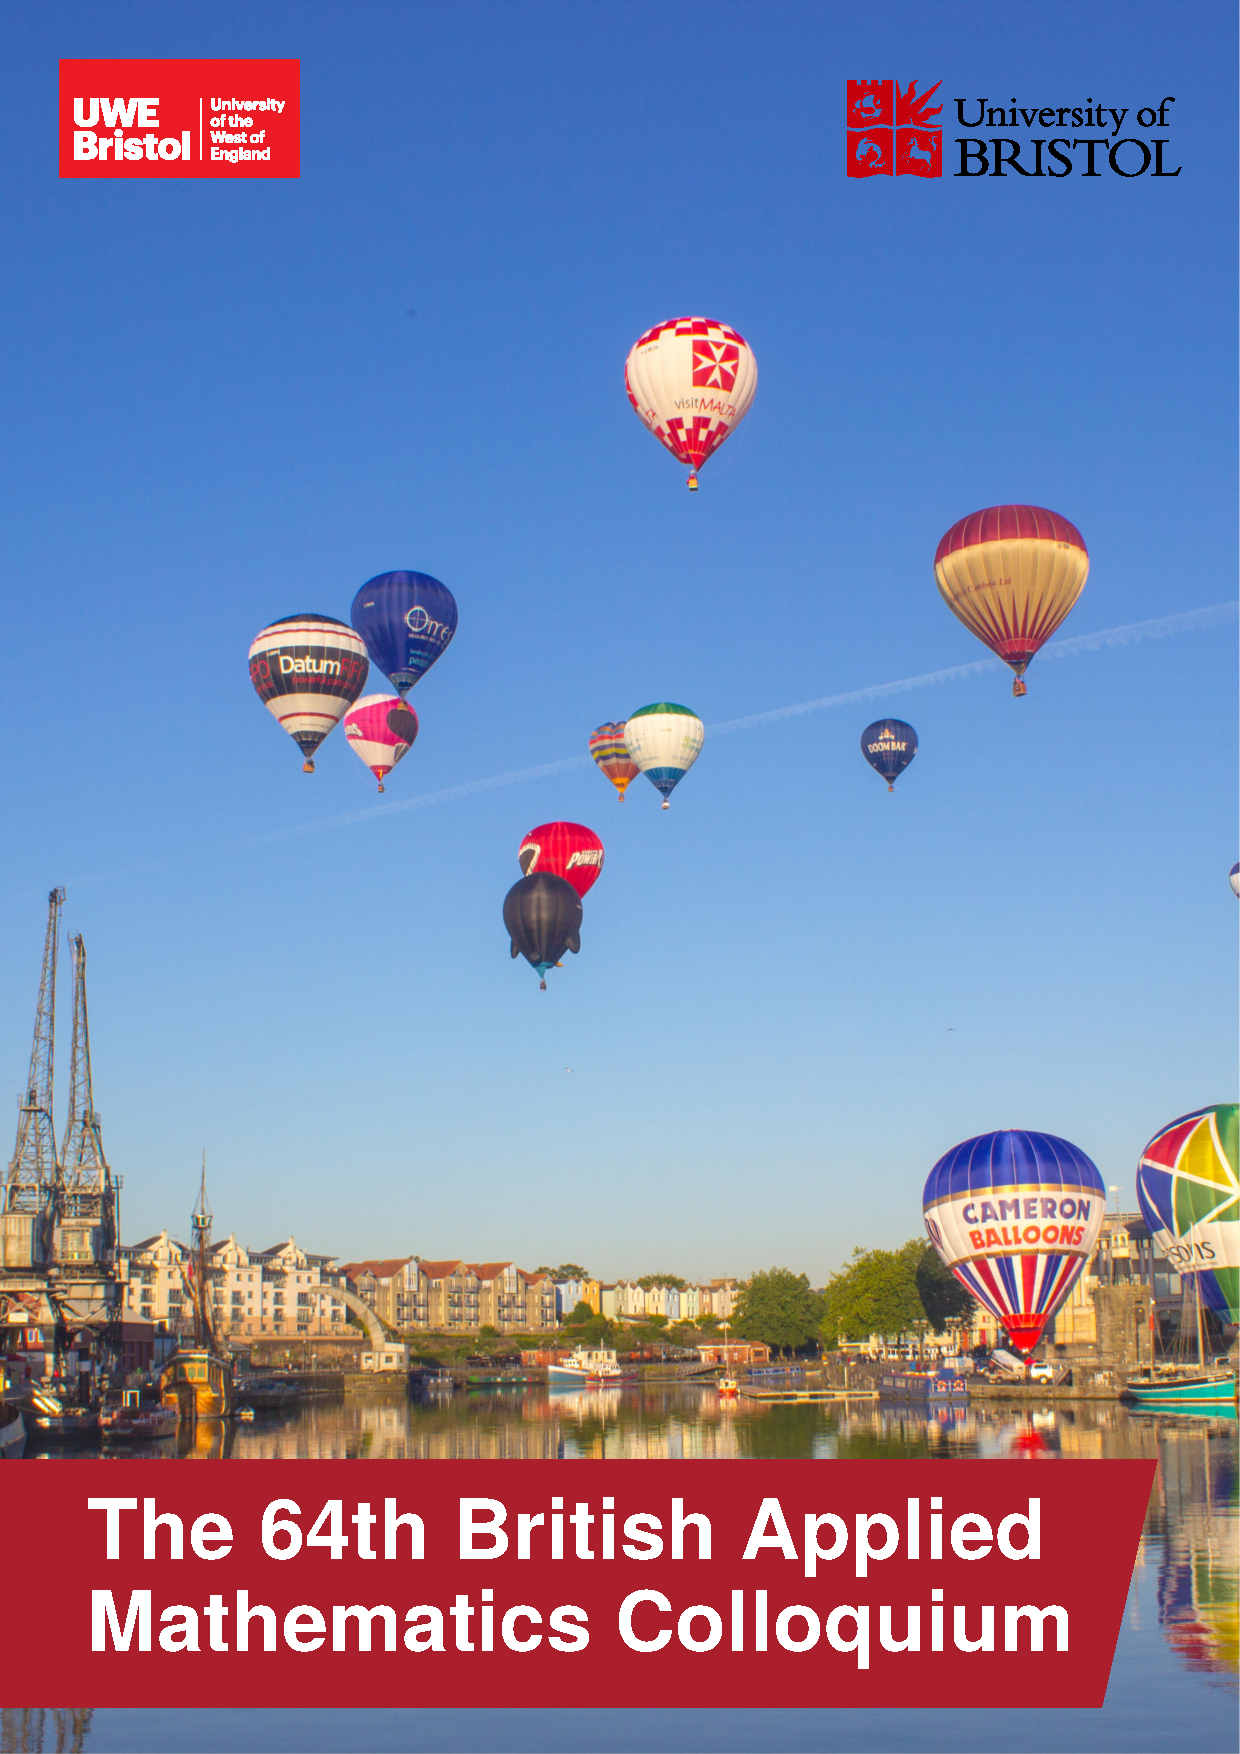
\includepdf{frontpage.pdf}
\setcounter{page}{1}

\section{Welcome}

\thispagestyle{empty}


\begin{tikzpicture}[remember picture,overlay,shift=(current page.south west)]
  \fill[UniversityRed, anchor=south west] rectangle (\paperwidth,4cm);
  \node[anchor=west] at (2, 2) {%
    \begin{minipage}{17cm}
      \color{white}\raggedright
      \textsc{\color{CoolGrey}\bfseries\large Organising Committee}
      \smallskip
    
      Cameron~Hall, Emily~Walsh, Lloyd~Bridge, Rachel~Long, Hemma~Philamore, Alan~Champneys, David~Barton, Eddie~Wilson
    \end{minipage}
  };
\end{tikzpicture}

\textcolor{DarkBlue}{\large Dear participants of the 64th BAMC, welcome to Bristol!}

It is with great pleasure that we welcome you to the 64th annual British Applied Mathematics Colloquium, hosted jointly by the Mathematics and Data Science Cluster located within the School of Computing and Creative Technologies at the University of the West of England (UWE) and the Department of Engineering Mathematics at the University of Bristol. This year's conference promises to be an exciting event, featuring a diverse range of talks and discussions on cutting-edge research in applied mathematics.

The BAMC has a long and distinguished history, and has become a key forum for researchers in the UK and beyond to exchange ideas and forge new collaborations. This year's conference continues that tradition, bringing together experts from a wide range of fields to explore the latest advances in applied mathematics, from fluid mechanics to data science and beyond.

We would like to express our thanks to all those who are contributing to this year's programme, including our plenary speakers, minisymposium organisers, and speakers. We hope that you will find the conference both enjoyable and informative, and that it will provide ample opportunity for networking, sharing ideas, and developing new collaborations. Once again, welcome to the 64th British Applied Mathematics Colloquium, and we look forward to seeing you over the next few days.

\section{Essential Information}

\subsection{Website and latest information}

The conference website is \href{https://bit.ly/bamc2023}{bit.ly/bamc2023}.

The online programme can be found at \href{https://bit.ly/bamc2023-programme}{bit.ly/bamc2023-programme}.

\subsection{Location}

The Colloquium is being hosted jointly by the University of the West of England Bristol, and the University of Bristol. It will be based at UWE Bristol Frenchay Campus With the public lecture and conference dinner taking place in Bristol city centre.

Address for Frenchay Campus: \textbf{Frenchay Campus, Coldharbour Lane, Bristol, BS16 1ZG}

\subsection{Taxis}

\begin{itemize}
\item \href{http://www.bristoldirectcars.co.uk/}{Bristol Direct Cars} \href{tel:01179651000}{0117 9651000}
\item \href{http://www.southgloscabs.co.uk/}{South Gloucestershire Taxis} \href{tel:01454320101}{01454 320101}
\item \href{https://www.eurotaxis.com/taxis/}{Euro taxis Ltd} \href{tel:03301621571}{0330 162 1571}
\end{itemize}

\subsection{Registration}

Registration will take place on 03 April from 09:00 in OneZone in E block on Frenchay Campus.

Look out for conference volunteers wearing orange lanyards to point you in the right direction.

\subsection{Refreshments and lunch}

Tea and coffee will be available throughout the conference in OneZone. There is also a Starbucks (OneZone) and the Atrium cafe (X block).

Lunch will be served in OneZone, you will be asked to show your conference name badge to gain entry, please ensure you have it with you throughout the conference. There will be a range of options, including vegan and gluten free, every day.

\subsection{Opening times}

\begin{itemize}
\item SU Bar: 12:00--18:00 3--6 April (food served between 12:00--17:30)
\item SU Shop: 8:00--18:00 3--6 April
\item Starbucks (OneZone): 08:00--18:00
\item Atrium café (X block): 08:00--15:00
\end{itemize}

\subsection{Food and drink in Bristol city centre}

Bristol has a fantastic range of restaurants and bars, many of which are located in the city centre and harbourside area. You will find many good options listed on the Visit Bristol website at \href{https://visitbristol.co.uk/food-and-drink}{visitbristol.co.uk/food-and-drink}.

Some specific suggestions are
\begin{itemize}
    \item Old City (around Baldwin Street): Ramen Monster, Burger Theory, Obento, BrewDog Bristol, Tuk Tuck, and Dangun
    \item Broad Quay: Turtle Bay, Pieminister, and Za Za Bazaar
    \item Stokes Croft: Pieminister, The Canteen, Om Burger, and Café Cuba
\end{itemize}

\subsection{Monday evening Poster Session and CUP wine reception}

This will take place in the Atrium Café (X Block), where the posters will be displayed throughout the conference. We encourage poster presenters to be beside their posters and able to answer questions throughout the Monday evening reception. Wine and non-alcoholic beverages will be available. The reception is being supported by Cambridge University Press (CUP).

\subsection{Public lecture}

The Public Lecture will take place at the University of Bristol's Priory Road Complex (12 Priory Road, Bristol BS8 1TU), on Tuesday 4 April. The lecture will commence at 17:30 with guest speaker Professor Zoe Doulgeri, Aristotle University of Thessaloniki, Greece. This lecture is included in your BAMC package, and you do not need to book separately. Coaches will be provided to transport you from UWE directly to the venue at University of Bristol.

\subsection{Conference Gala Dinner}

The conference gala dinner will take place at the Bristol Museum and Art Gallery, Queens Road, Bristol BS8 1RL. This is a short walk away from the plenary lecture in the Priory Road Lecture Theatre. Pre-dinner drinks are from 7pm and dinner is served at 8pm.

There will be a complementary pre-dinner drink and a bar is available for purchasing drinks throughout the evening. The bar will be open until 00:30.

The dinner is NOT included in the registration fee and must be booked separately.

\subsection{Mug}

There is a long standing tradition of a BAMC mug and this year is no different. A competition between local PhD students produced the winning design by Daniel Marris below.


\includegraphics[width=\linewidth]{MainMug.jpg}

From Daniel:
\begin{quote}
As a model of stochastic systems, lattice random walks have been employed for a long time, mainly by considering Cartesian lattices. However, in many applications, both for bounded and unbounded space, the geometry of the lattice has profound effects on the dynamics and ought to be accounted for. In my research, I mainly consider the cases of the six-neighbour (hexagonal) and three-neighbour (honeycomb) lattice, which have been seen in models ranging from adatoms diffusing in metals and excitations diffusing on single-walled carbon nanotubes to animal foraging strategy and the formation of territories in scent-marking organisms. By extending known techniques such as the Method of Images and the Defect Technique to these lattices I obtain analytic expressions for occupation probabilities and related transport quantities, such as the first passage to one or many targets, in bounded domains with different boundary conditions. A paper co-authored with Seeralan Sarvaharman and Luca Giuggioli is currently under review. 
\end{quote}

\subsection{Luggage}

Please notify the registration desk should you wish to leave luggage. Please note it is left at your own risk.

\subsection{Consent}

We will be taking photographs and may be making audio-visual recordings throughout the BAMC. When you register, you will be asked to give consent for these photographs and recordings to be used on our website as a record of the event and in promotional material for other future BAMC events and activities. You will have the opportunity to refuse consent. Please ensure that you make this clear when you register. Also please be prepared to sit towards the back of the lecture rooms to help us honour your wishes.

\subsection{Wi-Fi Access}

Wi-Fi is available anywhere on campus. If you have an existing eduroam account, you should automatically connect. 

If you do not have an eduroam account, there is a visitor cloud network (BT Free Wi-Fi).

\subsection{Contacts}

If you have any queries regarding the above then please do not hesitate to contact us at \href{mailto:researchevents@uwe.ac.uk}{researchevents@uwe.ac.uk}.

\subsection{COVID-19}

UWE Bristol are following Government guidelines, therefore mask wearing is at delegate's own discretion.

\section{Plenary Speakers}

\subsection{Prof.~Ian Griffiths, University of Oxford, UK}

\subsubsection{How can mathematics help us keep the world clean? (Stewartson Memorial Lecture)}

World cleaning applies to air, water and land: In the wake of the pandemic and the potential for future pandemics, how can we predict the risk of catching a virus in an indoor setting and how do antiviral air purifiers mitigate this risk?; The continued increase in water scarcity prompts us to seek better ways of providing clean water; And the novichok chemical warfare incident in 2018 motivates questions on how one adequately cleans up a chemical spill. In this talk, we use a variety of mathematical modelling techniques - some simple, others more complicated - to provide answers to these questions and others as we seek strategies to keep our world clean.

\subsubsection{Biography}

Ian Griffiths obtained his doctorate at the University of Oxford where he studied the mathematics of glass tube manufacture. He subsequently completed postdocs at Durham and Princeton University before become a Royal Society University Research Fellow at Oxford. His research accomplishments include modelling the performance of water filters for developing countries, which now serve more than 150,000 people, and producing mathematical models that are used in the design of Samsung and Huawei mobile phone screens. He is now a Professor of Industrial Mathematics at Oxford and the Janet Dyson Fellow of Mathematics at Mansfield College.

\subsection{Dr.~Adriana Dawes, Ohio State University, USA}

\subsubsection{Quantifying approximate symmetries in biological systems}

What do leaves and human faces have in common? What about daisies and sea urchins? They possess bilateral and rotational symmetries! Symmetry is a fundamental feature of natural systems, and is often correlated with survival, fecundity, and evolvability. While symmetry is ubiquitous and often intuitively obvious, symmetry in biological organisms is rarely perfect, making it challenging to apply mathematical definitions of idealized symmetry. To address this challenge, we developed a flexible, entropy-based method for quantifying symmetry that requires very little user input. I will highlight some novel insights arising from applications of this measure, including evidence for convergent evolution in flowering plants, classification of biopolymer networks, and visualization of the emergence and loss of symmetries in pattern formation systems.

\subsubsection{Biography}

Professor Dawes is a faculty member at the Ohio State University, with a joint appointment in the Department of Mathematics and the Department of Molecular Genetics. Prof. Dawes' research uses rigorous mathematical tools to uncover fundamental regulatory mechanisms in cell and developmental biology, with a particular focus on understanding how cells integrate biochemical, mechanical, and geometric information to make appropriate cell fate decisions. Prof. Dawes is a former Associate Director of the Mathematical Biosciences Institute, serves as senior editor at the Bulletin of Mathematical Biology, is the holder of a CAREER award from the National Science Foundation (USA), and is currently funded by the National Institutes of Health (USA).

Further information about the Dawes Lab: \href{https://people.math.osu.edu/dawes.33/}{https://people.math.osu.edu/dawes.33/}

\subsection{Dr.~Ellen Brooks Pollock, University of Bristol, UK}

\subsubsection{William Budd and 150 years of thinking about disease transmission}

William Budd was a physician at the Bristol Infirmary in the 19th century. He observed first-hand the devastating 1849 cholera epidemic in England and argued against prevailing miasma theory that infectious diseases were caused by foul smells, and instead made the case that an infectious agent was responsible. In this talk, I will re-examine Budd’s largely forgotten contribution to infectious disease theory and how he concluded that preventing transmission between infectious and susceptible individuals was the key to disease control. I will discuss approaches and challenges for describing disease transmission mathematically and how these ideas were used during the 2019 COVID pandemic to characterize transmission and shape the response. I will discuss methodology we developed during the pandemic to map social contact patterns to population—level epidemic metrics, and a specific example of modelling of COVID-19 transmission at the University of Bristol based on detailed social contact data.   
\subsubsection{Biography}

Ellen is an Associate Professor in Infectious Disease Modelling at the University of Bristol. She did an MSci in Mathematics at University College London in the previous century before completing her PhD on bovine tuberculosis and cattle movements at the University of Warwick. She has toured great institutions such as Harvard University, the London School of Hygiene and Tropical Medicine and the University of Cambridge before joining the University of Bristol as a lecturer in 2015. She is interested in developing data-driven models that challenge intuition and reveal truths about the world around us. She was heavily involved in the UK COVID modelling response for which she received an OBE in the 2021 Queen’s Birthday Honours list.  

\subsection{Prof.~Brian Wetton, University of British Columbia, Canada}

\subsubsection{Enthalpy Methods for Moving Boundary Problems}

We present the well understood Stefan and Oxygen Depletion Problems as examples of explicit and implicit moving boundary value problems respectively. We show the different ways these problems can be analyzed and computed numerically with a focus on the Enthalpy Method (a grid capturing technique). Generalized problems are shown, including two phase flow in porous media and the formation of sea ice. Rigorous analysis of the problems and their numerical approximation is missing in many of these generalized problems. 

\subsubsection{Biography}

Brian Wetton is a Professor in the Mathematics Department at the University of British Columbia. His awards include the 1992 NYU Kurt O. Friedrichs Prize, the 2000 Pacific Institute of Mathematical Sciences Industrial Outreach Prize, the 2008 UBC Alan Blizzard Award, and the 2010 CAIMS/MITACS Industrial Research Prize. The industrial mathematics awards were recognition of his leadership role in a fuel cell modelling project with Ballard Power Systems that had both industry and MITACS NCE funding. He was the director of the UBC Institute of Applied Mathematics (2013-2018). Mathematical modelling of electrochemical systems has been a major application of his modelling, asymptotic, and scientific computing skills: the expertise in this area has been applied to fuel cells, generalized dialysis devices, and currently Li-ion batteries.

\subsection{Prof.~James Gleeson, University of Limerick, Ireland}

\subsubsection{Data-driven modelling of cascades on networks (IMA Lighthill Lecture)}

Network models may be applied to describe many complex systems, and in the era of online social networks the study of dynamics on networks is an important branch of computational social science.  Cascade dynamics can occur when the state of a node is affected by the states of its neighbours in the network, for example when a Twitter user is inspired to retweet a message that she received from a user she follows, with one event (the retweet) potentially causing further events (retweets by followers of followers) in a chain reaction. In this talk I will review some mathematical models that can help us understand how social contagion (the spread of cultural fads and the viral diffusion of information) depends upon the structure of the social network and on the dynamics of human behaviour. Although the models are simple enough to allow for mathematical analysis, I will show examples where they can also provide good matches to empirical observations of cascades on social networks.

\subsubsection{Biography}

James Gleeson holds the Chair in Industrial and Applied Mathematics at the University of Limerick. As a member and former co-director of MACSI, the Mathematics Applications Consortium for Science and Industry, he leads research into applications of mathematics to real-world problems with significant economic and social impact. James is a graduate of University College Dublin in Mathematical Sciences and Mathematical Physics and received his PhD in Applied Mathematics from California Institute of Technology in 1999. Following his graduation from Caltech, he held positions as a visiting assistant professor in Arizona State University, postdoctoral research positions in the Department of Applied Mathematics at University College Cork (UCC) and National Microelectronic Research Centre (now Tyndall Institute) in Cork, and as a senior lecturer in the School of Mathematical Sciences, UCC before moving to Limerick in 2007. His research interests are in mathematical modelling, particularly of stochastic dynamics on complex networks.

\subsection{Prof.~Zoe Doulgeri, Aristotle University of Thessaloniki, Greece}

\subsubsection{Shared control in physical human-robot interaction applications (Public lecture)}

Over the last decades industrial robots have been widely deployed in the manufacturing industry, relieving workers from repetitive, unhealthy or arduous jobs with their workspace being strictly separated from that of humans for safety. Collaborative robots is a new generation of industrial robots that can work along side and with humans as co-workers or assistants. These robots are expected to provide flexibility by extending robot applications beyond the isolated structured work cells.  Collaborative robots should provide assistance to humans by reducing their physical and/or cognitive load, while being safe during their co-existence and collaboration with humans. In this talk, we will present shared control applications for resolving the problem of intentional physical human-robot interaction. The presentation will focus on the use of shared control methods for facilitating the human towards the kinesthetic teaching of a task, co-manipulating objects and progressive automation.

\subsubsection{Biography}

Zoe Doulgeri is a Professor of Robotics and Control of Manufacturing Systems and the director of the Automation and Robotics Lab of the Department of Electrical and Computer Engineering of the Aristotle University of Thessaloniki (AUTH). She received the diploma of Electrical Engineering from AUTH and an M.Sc. (DIC) in Control Systems, an M.Sc.(DIC)in Social and Economic Aspects of Science and Technology in Industry and a Ph.D in Mechanical Engineering, from the Imperial College, London, UK. She teaches Control Systems and Robotics. She authored more than 150 publications in peer-reviewed international journals and conferences. She is an evaluator of EU research and innovation proposals in Horizon-Europe and a reviewer in the most important robotics journals and conferences. She served as associate editor in the Journal of Intelligent and Robotic systems and the IEEΕ Robotics and Automation Letters. She has participated in many robotics projects financed by the EU and the Greek government. She has been the coordinator of the recently completed H2020 “Collaborate” project. She is currently coordinating an H2020European research project and two national projects. Her current research interests include the topics of physical human robot interaction, robot teaching and learning by demonstration, bimanual mobile robots, object grasping and manipulation with analytical and data based learning methods and the control of uncertain robotic systems. She has been the representative of Greece in the European Control Association from 2016-2021. She is a senior member of the IEEE, the IEEE Robotics and Automation Society and the IEEE Control Systems Society.

\section{Programme Overview}

Please see the online schedule at \href{https://bit.ly/bamc2023-programme}{bit.ly/bamc2023-programme} for the latest updates or for easier navigating on mobile devices.

\rowcolors{2}{BrightOrange!25}{BrightOrange!10}
\begin{tabularx}{\linewidth}{P{20mm}YP{50mm}}
  \rowcolor{BrightOrange}\multicolumn{3}{l}{\textcolor{white}{\bfseries\scshape Monday 3 April}}\\
  08:30--09:45 & Registration and coffee & OneZone (E block)\\
  09:45--10:00 & Welcome & X block lecture theatres*\\
  10:00--11:00 & Stewartson Memorial Lecture (Ian Griffiths) & X block lecture theatres*\\
  11:10--13:10 & Parallel sessions & Q block\\
  13:10--14:10 & Lunch & OneZone (E block)\\
  14:10--16:10 & Parallel sessions & Q block\\
  16:10--16:45 & Coffee & X block atrium\\
  16:45--17:45 & Plenary (Adriana Dawes) & X block lecture theatres*\\
  17:45--19:00 & Drinks reception sponsored by CUP & X block atrium
\end{tabularx}

\rowcolors{2}{BrightBlue!25}{BrightBlue!10}
\begin{tabularx}{\linewidth}{P{20mm}YP{50mm}}
  \rowcolor{BrightBlue}\multicolumn{3}{l}{\textcolor{white}{\bfseries\scshape Tuesday 4 April}}\\
  09:00--10:00 & Plenary (Ellen Brooks-Pollock) & X block lecture theatres*\\
  10:00--10:30 & Coffee & OneZone (E block)\\
  10:30--12:30 & Parallel sessions & Q block / E block\\
  12:30--13:30 & Lunch & OneZone (E block)\\
  13:30--15:30 & Parallel sessions & Q block\\
  15:30--16:00 & Coffee & X block atrium\\
  16:00--17:30 & Travel for public lecture & \\
  17:30--18:30 & Public lecture (Zoe Doulgeri) & Priory Road lecture theatre\\
  19:00 & Conference dinner & Bristol Museum and Art Gallery
\end{tabularx}

\rowcolors{2}{BrightPurple!25}{BrightPurple!10}
\begin{tabularx}{\linewidth}{P{20mm}YP{50mm}}
  \rowcolor{BrightPurple}\multicolumn{3}{l}{\textcolor{white}{\bfseries\scshape Wednesday 5 April}}\\
  09:00--10:00 & Plenary (Brian Wetton) & X block lecture theatres*\\
  10:00--10:30 & Coffee & OneZone (E block) \\
  10:30--12:30 & Parallel sessions & Q block / E block\\
  12:30--13:30 & Lunch & OneZone (E block)\\
  13:30--14:30 & Lighthill Lecture (James Gleeson) & X block lecture theatres*\\
  14:30--15:00 & Closing & X block lecture theatres*
\end{tabularx}

Tea and coffee will be available throughout the conference in OneZone (E block)

*The conference opening, closing, and plenaries will all be held in the 2X112 lecture theatre. This will not have the capacity for all conference participants and there will be a spillover room in 2X242.

\section{Overview of Parallel Sessions}

\begin{tabularx}{\linewidth}{P{12mm}YYYYY}
  \cellcolor{CoolGrey!50!black}\textbf{\color{white}Room} & \cellcolor{BrightOrange}\textbf{\color{white}Monday AM} & \cellcolor{BrightOrange}\textbf{\color{white}Monday PM} & \cellcolor{BrightBlue}\textbf{\color{white}Tuesday AM} & \cellcolor{BrightBlue}\textbf{\color{white}Tuesday PM} & \cellcolor{BrightPurple}\textbf{\color{white}Wednesday AM}\\
  \cellcolor{CoolGrey!50}2Q42 & \cellcolor{BrightOrange!10}{Advances in water waves and free-surface flows I} & \cellcolor{BrightOrange!10}{Advances in water waves and free-surface flows II} & \cellcolor{BrightBlue!10}{Mathematical modelling in sport} & \cellcolor{BrightBlue!10}{Sea ice modelling} & \cellcolor{BrightPurple!10}{Mathematical modelling of sleep and circadian rhythms: from molecular mechanisms to policy}\\
  \cellcolor{CoolGrey}2Q48 & \cellcolor{BrightOrange!25}{Mechanics of hydrogels and poroelastic media} & \cellcolor{BrightOrange!25}{Controlling active matter} & \cellcolor{BrightBlue!25}{Advances in applied numerical linear algebra and its applications} & \cellcolor{BrightBlue!25}{\itshape Self-propulsion and fluid-body interactions} & \cellcolor{BrightPurple!25}{Optimisation and control for nonlinear dynamics}\\
  \cellcolor{CoolGrey!50}2Q49 & \cellcolor{BrightOrange!10}{Dynamics of reaction-transport systems I} & \cellcolor{BrightOrange!10}{Dynamics of reaction-transport systems II} & \cellcolor{BrightBlue!10}{IMA Lighthill-Thwaites prize I} & \cellcolor{BrightBlue!10}{IMA Lighthill-Thwaites prize II} & \cellcolor{BrightPurple!10}{Networks and complex systems in society}\\
  \cellcolor{CoolGrey}2Q50/51 & \cellcolor{BrightOrange!25}{Preparation for future pandemics: Recent lessons} & \cellcolor{BrightOrange!25}{Mathematical pharmacology} & \cellcolor{BrightBlue!25}{Neurodynamics} & \cellcolor{BrightBlue!25}{Modelling and inference in public health} & \cellcolor{BrightPurple!25}{\itshape Epidemiology and statistical learning}\\
  \cellcolor{CoolGrey!50}3Q16 & \cellcolor{BrightOrange!10}{\itshape Game theory and agent based models} & \cellcolor{BrightOrange!10}{\itshape Mathematical ecology} & \cellcolor{BrightBlue!10}{\itshape Collective behaviour and transport} & \cellcolor{BrightBlue!10}{\itshape Stochastic processes and random walks} & \cellcolor{BrightPurple!10}{\itshape Evaporation}\\
  \cellcolor{CoolGrey}3Q68 & \cellcolor{BrightOrange!25}{\itshape Cell modelling} & \cellcolor{BrightOrange!25}{\itshape Cell and tissue mechanics} & \cellcolor{BrightBlue!25}{\itshape Mathematical medicine} & \cellcolor{BrightBlue!25}{\itshape Biofilms and pattern formation} & \cellcolor{BrightPurple!25}{\itshape Blood and blood vessels}\\
  \cellcolor{CoolGrey!50}4Q04 & \cellcolor{BrightOrange!10}{\itshape Droplets and impact} & \cellcolor{BrightOrange!10}{\itshape Numerical methods} & \cellcolor{BrightBlue!10}{\itshape Complex systems and control} & \cellcolor{BrightBlue!10}{\itshape Travelling waves} & \cellcolor{BrightPurple!10}{\itshape Nonlinear dynamics and applications}\\
  \cellcolor{CoolGrey}4Q05 & \cellcolor{BrightOrange!25}{\itshape Acoustics} & \cellcolor{BrightOrange!25}{\itshape Solid mechanics} & \cellcolor{BrightBlue!25}{Multiple wave scattering I} & \cellcolor{BrightBlue!25}{Multiple wave scattering II} & \cellcolor{BrightPurple!25}{Metamaterial modelling and design}\\
  \cellcolor{CoolGrey!50}4Q07 & \cellcolor{BrightOrange!10}{\itshape Mathematics of energy} & \cellcolor{BrightOrange!10}{\itshape Neurons and networks} & \cellcolor{BrightBlue!10}{\itshape Geophysics and climate} & \cellcolor{BrightBlue!10}{\itshape Industrial mathematics} & \cellcolor{BrightPurple!10}{\itshape Granular and multiphase flows}\\
  \cellcolor{CoolGrey}4Q08 & \cellcolor{BrightOrange!25}{\itshape Analysis of continuum mechanics} & \cellcolor{BrightOrange!25}{\itshape Boundary layer flows and stability} & \cellcolor{BrightBlue!25}{\itshape Thin films and contact lines} & \cellcolor{BrightBlue!25}{\itshape Microfluidics and flow in porous media} & \cellcolor{BrightPurple!25}{\itshape Filaments, membranes, and shells}\\
  \cellcolor{CoolGrey!50}4Q56 & \cellcolor{BrightOrange!10}{Physiological flows and transport} & \cellcolor{BrightOrange!10}{Mathematical and computational ophthalmology} & \cellcolor{BrightBlue!10}{Chemo-mechanical couplings in growing tissues} & \cellcolor{BrightBlue!10}{New mathematical approaches in the life sciences} & \cellcolor{BrightPurple!10}{Asymptotics in active matter}\\
  \cellcolor{CoolGrey}3E11 & \cellcolor{BrightOrange!25}{} & \cellcolor{BrightOrange!25}{} & \cellcolor{BrightBlue!25}{\itshape Liquid crystals and transport models} & \cellcolor{BrightBlue!25}{} & \cellcolor{BrightPurple!25}{\itshape Applied fluid dynamics}
\end{tabularx}

Contributed talks sessions are denoted in \textit{italics}.

\section{Minisymposia Sessions}

\subsection{Monday 11:10–13:10}

\rowcolors{2}{BrightOrange!25}{BrightOrange!10}
\begin{tabularx}{\linewidth}{C{15mm}YP{50mm}}
\rowcolor{BrightOrange}\textcolor{white}{\textbf{2Q42}} & & \\
& \textbf{Advances in water waves and free-surface flows} & \\
11:10 & Water waves with vorticity and the Schwarz function & Darren Crowdy\\
11:30 & Exact solutions for submerged von Kármán point vortex streets cotravelling with a wave on a linear shear cuurent & Jack Keeler, Darren Crowdy\\
11:50 & On Ostrovsky-type models & Karima Khusnutdinova, Matthew Tranter\\
12:10 & Incipient wave breaking within higher-order spectral methods & Tatjana Kokina, J N Steer, S A Hasan, F Dias\\
12:30 & Desingularization and global continuation for hollow vortices & Miles Wheeler, Robin Ming Chen, Samuel Walsh\\
12:50 & Interfacial gravity waves and their limiting configurations & Xin Guan, Jean-Marc Vanden-Broeck\\
\end{tabularx}

\rowcolors{2}{BrightOrange!25}{BrightOrange!10}
\begin{tabularx}{\linewidth}{C{15mm}YP{50mm}}
\rowcolor{BrightOrange}\textcolor{white}{\textbf{2Q48}} & & \\
& \textbf{Mechanics of hydrogels and poroelastic media} & \\
11:10 & Multiscale modelling of a fibrous bioreactor scaffold & Amy Kent, James Oliver, Sarah Waters, Jon Chapman\\
11:30 & Formation and collapse of gas cavities in a soft porous medium & Oliver Paulin, Liam Morrow, Matthew Hennessy, Christopher MacMinn\\
11:50 & Multiple scales homogenisation of a porous viscoelastic material with rigid inclusions & Andres F Galvis, J M Foster, Bartosz Protas, Stephen J Chapman\\
12:10 & Swelling-induced folds in soft microchannels & Haolin Li, Aidan Retallick, Anne Juel, Matthias Heil, Draga Pihler-Puzovic\\
12:30 & Computational Modelling of stimuli-responsive hydrogels & Amin Rahmat, Mostafa Safdari Shadloo, Tom Montenegro-Johnson\\
12:50 & Curvature-controlled beading in stretched hydrogel cylinders & Matteo Taffetani, Matthew Hennessy\\
\end{tabularx}

\rowcolors{2}{BrightOrange!25}{BrightOrange!10}
\begin{tabularx}{\linewidth}{C{15mm}YP{50mm}}
\rowcolor{BrightOrange}\textcolor{white}{\textbf{2Q49}} & & \\
& \textbf{Dynamics of reaction-transport systems} & \\
11:10 & VisualPDE: Using WebGL to Rapidly Explore PDE Dynamics for Fun and Profit & Andrew Krause, Benjamin Walker, Adam Townsend\\
11:50 & Reaction-Transport Dynamics in the Decontamination of Porous Media & Ellen Luckins\\
12:10 & Pattern Formation in a Nonlocal Model for Cell Attraction and Repulsion in 2 or More Dimensions & Thomas Jun Jewell, Andrew L Krause, Philip K Maini, Eamonn A Gaffney\\
12:30 & Pattern formation in multiphase, moving boundary models of tissue growth & Jacob Jepson, John Billingham, Reuben O'Dea, Nabil Fadai\\
12:50 & Minimal reaction schemes for Turing instabilities & Fraser Waters, Kit Yates, Jonathan Dawes\\
\end{tabularx}

\rowcolors{2}{BrightOrange!25}{BrightOrange!10}
\begin{tabularx}{\linewidth}{C{15mm}YP{50mm}}
\rowcolor{BrightOrange}\textcolor{white}{\textbf{2Q50/51}} & & \\
& \textbf{How to be better prepared for a future pandemic: lessons learned from COVID-19, mpox and the four historic influenza pandemics} & \\
11:10 & Importance of progressive transmissibility of emerging variants in sustaining the COVID-19 epidemic in England & Ben Swallow\\
11:30 & The interplay between population susceptibility and vaccine effectiveness control the timing and size of an emerging influenza wave & Edwin Van Leeuwen\\
11:50 & Considerations for informing Test, Trace and support to Isolate (TTI) intervention design following the experience of COVID-19 & Elizabeth Fearon\\
12:10 & The role of enclosed population in an epidemic  & Thomas Finnie\\
12:30 & WasteWater as a pandemic surveillance tool & Zhou Fang\\
12:50 & Lessons from modelling during a pandemic and for pandemic preparedness  & Jasmina Panovska-Griffiths\\
\end{tabularx}

\rowcolors{2}{BrightOrange!25}{BrightOrange!10}
\begin{tabularx}{\linewidth}{C{15mm}YP{50mm}}
\rowcolor{BrightOrange}\textcolor{white}{\textbf{4Q56}} & & \\
& \textbf{Physiological flows and transport} & \\
11:10 & Generalised tube laws for the deformation of elastic-walled tubes with arbitrary cross-sections & Daniel Netherwood, Robert J Whittaker\\
11:30 & Understanding the mechanism of unconventional drainage from the eye & Jennifer Tweedy, Mariia Dvoriashyna, Jessica Crawshaw, Darryl Overby, Rodolfo Repetto, Paul Roberts, Tamsin Spelman, Peter Stewart, Alexander Foss\\
11:50 & Modelling oxygen transport in the human cerebral microvasculature & Yidan Xue, Stephen Payne\\
12:10 & Modelling metabolite transport in hollow fibre membrane bioreactors & George Booth, Mohit Dalwadi, Pierre-Alexis Mouthuy, Hua Ye, Sarah Waters\\
12:30 & Flow and transport in the human placenta: from multiscale imaging to structural determinants of function & Igor Chernyavsky, Alys Clark, Alexander Erlich, Oliver Jensen, Philip Pearce, Win Tun, Carl Whitfield, et al.\\
12:50 & Oscillatory and steady streaming flow of cerebrospinal fluid during the cardiac cycle & Mariia Dvoriashyna, Alain Goriely\\
\end{tabularx}

\subsection{Monday 14:10–16:10}

\rowcolors{2}{BrightOrange!25}{BrightOrange!10}
\begin{tabularx}{\linewidth}{C{15mm}YP{50mm}}
\rowcolor{BrightOrange}\textcolor{white}{\textbf{2Q42}} & & \\
& \textbf{Advances in water waves and free-surface flows} & \\
14:10 & Modulational instability and recurrence of hydrodynamic waves with frequency-dependent dissipation & Alberto Alberello, Emilian Parau\\
14:30 & A thin plate approximation for thick floating ice & Luke Bennetts\\
14:50 & Ship wave patterns on floating ice sheets & Emilian Parau\\
15:10 & The nonlinear Benjamin-Feir instability - a discrete Hamiltonian approach & Raphael Stuhlmeier, David Andrade\\
15:30 & Exponential asymptotics for the Saffman-Taylor problem in a wedge & Cecilie Andersen, Chris Lustri, Scott McCue, Phil Trinh\\
15:50 & Three dimensional hydroelastic solitary waves  in shallow water & Yanghan Meng, Zhan Wang\\
\end{tabularx}

\rowcolors{2}{BrightOrange!25}{BrightOrange!10}
\begin{tabularx}{\linewidth}{C{15mm}YP{50mm}}
\rowcolor{BrightOrange}\textcolor{white}{\textbf{2Q48}} & & \\
& \textbf{Controlling active matter} & \\
14:10 & Odd dynamics of living chiral crystals & Alexander Mietke, T H Tan, J Li, Y Chen, H Higinbotham, P J Foster, S Gokhale, J Dunkel, N Fakhri\\
14:30 & Conditions for hydrodynamic coordination in arrays of model cilia & Rachel Bennett, Fanlong Meng, Nariya Uchida, Ramin Golestanian\\
14:50 & Is the tendency for all living systems to do work universal? & Elsen Tjhung\\
15:10 & Shear thickening and Yielding Transitions in Biological Tissues & Michael Hertaeg, Suzanne Fielding, Dapeng Bi\\
15:30 & Active elastocapillarity in soft solids with negative surface tension & Jack Binysh, Thomas R Wilks, Anton Souslov\\
15:50 & Large deviations and optimal control in active fluids & Robert Jack\\
\end{tabularx}

\rowcolors{2}{BrightOrange!25}{BrightOrange!10}
\begin{tabularx}{\linewidth}{C{15mm}YP{50mm}}
\rowcolor{BrightOrange}\textcolor{white}{\textbf{2Q49}} & & \\
& \textbf{Dynamics of reaction-transport systems} & \\
14:10 & Pattern Formation on a Finite Disk, Variational and Non Variational Case & Nicolas Verschueren van Rees, Edgar Knobloch, Hannes Uecker\\
14:30 & Understanding fully localised 2D patterns with dihedral symmetry & Dan J Hill, Jason J Bramburger, David J B Lloyd\\
14:50 & Homoclinic snaking \& localised patterns beyond all asymptotic orders & Edgardo Villar-Sepúlveda, Alan Champneys\\
15:10 & Nonlocal models of cell-cell adhesion and their Cahn-Hilliard approximation & Carles Falcó, Ruth E Baker, José A Carrillo\\
15:30 & Stability and multi-stability in non-local advection-diffusion models & Valeria Giunta, Thomas Hillen, Mark Lewis, Jonathan Potts\\
15:50 & Self-organised patterning in Dictyostelium group migration & Giulia Celora, Hugh Ford, Mohit Dalwadi, Benjamin Walker, Jonathan Chubb, Philip Pearce\\
\end{tabularx}

\rowcolors{2}{BrightOrange!25}{BrightOrange!10}
\begin{tabularx}{\linewidth}{C{15mm}YP{50mm}}
\rowcolor{BrightOrange}\textcolor{white}{\textbf{2Q50/51}} & & \\
& \textbf{Mathematical pharmacology} & \\
14:10 & Practical application of quantitative systems toxicology models in drug development: learnings and case studies from the IMI2-tQST project & Ciarán Fisher\\
14:50 & Extensions of receptor theory to include dimerised and dimerising receptor dynamics & Lloyd Bridge, Carla White\\
15:10 & Physiologically-Based Pharmacokinetic Modelling: The Double-Edged Sword of Complexity & Aleksandra Kmieciak\\
15:30 & Cybergenetics applications in mammalian cells: closing the loop on non-linear dynamics & Lucia Marucci\\
15:50 & Structural Identifiability Analysis: A Tool for Mathematical Pharmacology & Michael Chappell, Neil D Evans\\
\end{tabularx}

\rowcolors{2}{BrightOrange!25}{BrightOrange!10}
\begin{tabularx}{\linewidth}{C{15mm}YP{50mm}}
\rowcolor{BrightOrange}\textcolor{white}{\textbf{4Q56}} & & \\
& \textbf{Mathematical and computational ophthalmology} & \\
14:10 & Mathematical and Computational Ophthalmology: Coming of Age & Paul A Roberts\\
14:30 & A tool for automated retinal vascular morphology quantification and its applications & Yukun Zhou, Daniel Alexander, Pearse Keane\\
14:50 & Pressure wave transmission across the lamina cribrosa & Peter Stewart, Ifeanyi Sunday Onah, David MacTaggart\\
15:10 & High amplitude elastic jump propagation through blood vessel junctions  & Tamsin A Spelman, Ifeanyi S Onah, David MacTaggart, Peter S Stewart\\
15:30 & Characterising eyes with neovascular age-related macular degeneration & Remi Hernandez\\
15:50 & The important role of hierarchical Bayesian inference in understanding macular degeneration treatment strategies & Jessica Crawshaw, Eamonn Gaffney, Philip Maini, Antonello Caruso, Michael Gertz\\
\end{tabularx}

\subsection{Tuesday 10:30–12:30}

\rowcolors{2}{BrightBlue!25}{BrightBlue!10}
\begin{tabularx}{\linewidth}{C{15mm}YP{50mm}}
\rowcolor{BrightBlue}\textcolor{white}{\textbf{2Q42}} & & \\
& \textbf{Mathematical modelling in sport} & \\
10:30 & Gunwale bobbing and the effect of heave and pitch during a rowing race & Graham P Benham\\
10:50 & Improving the self-stability of a bicycle via spectral abscissa minimisation & Oleg Kirillov\\
11:10 & Effects of friction and tangential compliance in golf ball bounce & Stanislaw W Biber, Alan R Champneys, Robert Szalai\\
11:30 & Alpine pendulum & Serguei Komissarov\\
11:50 & Analysis of Soccer Ball Collision Kinematics and Kinetics Using Image Processing Techniques & Ieuan Phillips, Andy Harland, Séan Mitchell, Paul Lepper\\
12:10 & Exploration into the spatial and temporal movement of the female breast during motion. & Lauren Holmes, Andy Harland\\
\end{tabularx}

\rowcolors{2}{BrightBlue!25}{BrightBlue!10}
\begin{tabularx}{\linewidth}{C{15mm}YP{50mm}}
\rowcolor{BrightBlue}\textcolor{white}{\textbf{2Q48}} & & \\
& \textbf{Advances in applied numerical linear algebra and its applications} & \\
10:30 & Flexible and inexact Krylov methods for inverse problems & Malena Sabaté Landman\\
11:10 & Applied Krylov subspace algorithms in CT using the TIGRE toolbox & Ander Biguri, Malena Sabate Landman, Sepideh Hatamikia, Richard Boardman, John Aston, Carola-Bibiane Schonlieb\\
11:30 & Structure-Exploiting Preconditioners for Data Assimilation & Jemima Tabeart, John W Pearson, Selime Gürol, Anthony Weaver\\
11:50 & Model Based Iterative Reconstruction of Tomographic data with the Core Imaging Library & Edoardo Pasca, Evelina Ametova, Gemma Fardell, Jakob Sauer Jørgensen, Laura Murgatroyd, Evangelos Papoutsellis\\
12:10 & Data-Driven Mirror Descent with Input-Convex Neural Networks & Subhadip Mukherjee, Hong Ye Tan, Junqi Tang, Andreas Hauptmann, Carola-Bibiane Schönlieb\\
\end{tabularx}

\rowcolors{2}{BrightBlue!25}{BrightBlue!10}
\begin{tabularx}{\linewidth}{C{15mm}YP{50mm}}
\rowcolor{BrightBlue}\textcolor{white}{\textbf{2Q49}} & & \\
& \textbf{IMA Lighthill-Thwaites prize} & \\
10:50 & Modelling melting, structure and microbial activity of an ice sheet surface & Tilly Woods, Ian Hewitt\\
11:10 & Exponential asymptotics for steady capillary ripples on steep gravity waves & Josh Shelton\\
11:30 & On the deformation of an elastic particle under pressure-driven axisymmetric channel flow & Simon M Finney, Matthew G Hennessy, Andreas Muench, Sarah Waters\\
11:50 & Matched asymptotics, conformal capacity, and applications & Hiroyuki Miyoshi, Darren G Crowdy\\
12:10 & Controlling stratification in drying films with diffusiophoresis & Clare Rees-Zimmerman, Alex Routh\\
\end{tabularx}

\rowcolors{2}{BrightBlue!25}{BrightBlue!10}
\begin{tabularx}{\linewidth}{C{15mm}YP{50mm}}
\rowcolor{BrightBlue}\textcolor{white}{\textbf{2Q50/51}} & & \\
& \textbf{Neurodynamics} & \\
10:30 & Modeling Alzheimer's progression: Oscillator dynamics on evolving networks & Christoffer Gretarsson Alexandersen, Alain Goriely, Christian Bick, Willem de Haan\\
10:50 & Phase-Isostable Reduction of Coupled Oscillator Networks & Robert Allen\\
11:10 & Exploring the bifurcations of excitable cells with control-based continuation & Mark Blyth, Krasimira Tsaneva-Atanasova, Kyle Wedgwood, Lucia Marucci, Ludovic Renson\\
11:30 & Tonic-clonic seizure transitions in a next generation neural field model & Oliver Cattell\\
11:50 & Hierarchical processing underpins competition in tactile perceptual bistability & Farzaneh Darki, Andrea Ferrario, James Rankin\\
12:10 & Investigating travelling waves in a 2D network of spiking neurons & Henry Kerr\\
\end{tabularx}

\rowcolors{2}{BrightBlue!25}{BrightBlue!10}
\begin{tabularx}{\linewidth}{C{15mm}YP{50mm}}
\rowcolor{BrightBlue}\textcolor{white}{\textbf{4Q05}} & & \\
& \textbf{Multiple wave scattering} & \\
10:30 & Multiple scattering in the spirit of Leslie Foldy & Paul Martin\\
11:10 & High-frequency homogenization for dispersive materials of the Lorentz type & Marie Touboul, R Assier, R Craster, S Guenneau, B Vial\\
11:30 & Diffraction by a finite barrier/crack on a square lattice: an iterative Wiener-Hopf method approach & Elena Medvedeva, Anastasia Kisil, Raphael Assier\\
11:50 & Effects of gravity and dispersive waves in chiral elastic systems & Alessio Kandiah, Ian S Jones, Natasha V Movchan, Alexander B Movchan\\
12:10 & Time-dependent problems in Wave Scattering & Michael Meylan\\
\end{tabularx}

\rowcolors{2}{BrightBlue!25}{BrightBlue!10}
\begin{tabularx}{\linewidth}{C{15mm}YP{50mm}}
\rowcolor{BrightBlue}\textcolor{white}{\textbf{4Q56}} & & \\
& \textbf{Chemo-mechanical couplings in growing tissues} & \\
10:30 & A patient-specific framework for studying the influence of chemo-mechanical cues on brain tumour growth and surrounding healthy tissue damage. & Chiara Giverso, Francesca Ballatore, Giulio Lucci\\
11:10 & Minimal Morphoelastic Models of Solid Tumour Spheroids & Benjamin Walker, Giulia L Celora, Alain Goriely, Derek E Moulton, Helen M Byrne\\
11:30 & The effects of non-local diffusion on the growth of an avascular tumour & Ariel Ramirez Torres, Mariam Al Mudarra, Alfio Grillo\\
11:50 & Mechanotransduction in axon: Remodelling of the actin cortex & Davide Riccobelli, D Andrini, V Balbi, G Bevilacqua, G Lucci, G Pozzi\\
12:10 & Mechanical feedback in size regulation & Alexander Erlich, Pierre Recho\\
\end{tabularx}

\subsection{Tuesday 13:30–15:30}

\rowcolors{2}{BrightBlue!25}{BrightBlue!10}
\begin{tabularx}{\linewidth}{C{15mm}YP{50mm}}
\rowcolor{BrightBlue}\textcolor{white}{\textbf{2Q42}} & & \\
& \textbf{Sea ice modelling} & \\
13:30 & From Micro to Macro in Sea Ice Modelling & Kenneth M Golden\\
14:10 & Partial Differential Equation Models and Deep Learning for the Sea Ice Concentration Field & Delaney Mosier\\
14:30 & Seasonal evolution of the Arctic sea ice thickness distribution & Srikanth Toppaladoddi, Woosok Moon, John S Wettlaufer\\
14:50 & A computational model of the freezing of salt water  & Brian Wetton\\
15:10 & Dynamics of Brine Inclusions in First Year Sea Ice & Keith Promislow, Noa Kraitzman, Yuan Chen, Brian Wetton\\
\end{tabularx}

\rowcolors{2}{BrightBlue!25}{BrightBlue!10}
\begin{tabularx}{\linewidth}{C{15mm}YP{50mm}}
\rowcolor{BrightBlue}\textcolor{white}{\textbf{2Q49}} & & \\
& \textbf{IMA Lighthill-Thwaites prize} & \\
13:30 & Nonlinear waves in viscous multilayer shear flows in the presence of interfacial slip & Anna Katsiavria, Demetrios T Papageorgiou\\
13:50 & A two-complex-variable approach to the right-angled no-contrast penetrable wedge diffraction problem & Valentin Kunz, Raphael Assier\\
14:10 & Data-driven discovery of PDEs & Nicolas Boullé, Alex Townsend\\
\end{tabularx}

\rowcolors{2}{BrightBlue!25}{BrightBlue!10}
\begin{tabularx}{\linewidth}{C{15mm}YP{50mm}}
\rowcolor{BrightBlue}\textcolor{white}{\textbf{2Q50/51}} & & \\
& \textbf{Modelling and inference in public health} & \\
13:30 & Bayesian multilevel modelling for prediction and uncertainty estimation of motor progression in Parkinson's disease & Tanja Zerenner, Michael Lawton, Anahita Nodehi, Donald Grosset \& the Tracking Parkinson’s team, Michele Hu \& the OPDC-Discovery team, Yoav Ben-Shlomo\\
13:50 & The role of large connected components in sexual networks for HIV spreading in Sub-Saharan Africa & Francesco Di Lauro\\
14:10 & How data-driven, mechanistic modelling is being used to support elimination of African sleeping sickness  & Kat S Rock\\
14:30 & Combining models to generate consensus nowcasts for the COVID-19 epidemic status in England & Harrison Manley, Josie Park, Luke Bevan, Alberto Sanchez-Marroquin, Gabriel Danelian, Thomas Bayley, Veronica Bowman, Thomas Maishman, Thomas Finnie, Andre Charlett, Nicholas A Watkins, Johanna Hutchinson, Steven Riley, Jasmina Panovska-Griffiths, Sebastian Funk, Paul Birrell, Daniela De Angelis, Matt Keeling, Lorenzo Pellis, Marc Baguelin, Graeme Ackland, Jonathan Read, Christopher Jewell, Robert Challen\\
14:50 & The observational model: a data-driven parameter estimation technique for dynamical systems & James Van Yperen, Eduard Campillo-Funollet, Anotida Madzvamuse\\
\end{tabularx}

\rowcolors{2}{BrightBlue!25}{BrightBlue!10}
\begin{tabularx}{\linewidth}{C{15mm}YP{50mm}}
\rowcolor{BrightBlue}\textcolor{white}{\textbf{4Q05}} & & \\
& \textbf{Multiple wave scattering} & \\
13:30 & Full Waveform Inversion via Reduced Order Modeling & Josselin Garnier, Liliana Borcea, Alexander Mamonov, Jorn Zimmerling\\
13:50 & Wave Scattering from Layers of Random Particulate Materials & Paulo Sergio Piva, Kevish K Napal, Artur L Gower\\
14:10 & Using elastic waves to predict forces in thick-walled cylinder with application to roller-bearings & Jessica Jordan Kent, Artur Lewis Gower\\
14:30 & Causality Constraint as a Design Tool for Sound Absorption Metastructures & Ping Sheng\\
14:50 & Multiple wave scattering in soft complex media & Valerie J Pinfield\\
15:10 & Spectral convergence of defect modes in large finite resonator arrays & Bryn Davies\\
\end{tabularx}

\rowcolors{2}{BrightBlue!25}{BrightBlue!10}
\begin{tabularx}{\linewidth}{C{15mm}YP{50mm}}
\rowcolor{BrightBlue}\textcolor{white}{\textbf{4Q56}} & & \\
& \textbf{New mathematical approaches in the life sciences} & \\
13:30 & Exploring electrical environments: the unique sense of electroreception & Ryan Palmer, Isaac V Chenchiah, Daniel Robert\\
13:50 & Extended Pair Correlation Functions for Multiplex Medical Imaging & Joshua A Bull, Helen M Byrne\\
14:10 & Mathematics, the Mind and Alzheimer's disease: Systematical progression on brain graphs & Prama Putra, Alain Goriely\\
14:30 & Field Theories of Branching in Cell Populations, Epidemiology and Neuronal Signals & Johannes Pausch\\
14:50 & Viral geometry as a key to understanding viral infections & Reidun Twarock\\
15:10 & Mathematical and deep learning analysis of wound healing in flies & Jake Turley, I V Chenchiah, T B Liverpool, H Weavers, P Martin\\
\end{tabularx}

\subsection{Wednesday 10:30–12:30}

\rowcolors{2}{BrightPurple!25}{BrightPurple!10}
\begin{tabularx}{\linewidth}{C{15mm}YP{50mm}}
\rowcolor{BrightPurple}\textcolor{white}{\textbf{2Q42}} & & \\
& \textbf{Mathematical modelling of sleep and circadian rhythms: from molecular mechanisms to policy} & \\
10:30 & Mathematical modelling of the wheat circadian clock & Abhishek Upadhyay, Jamila Rowland-Chandler, Gabriela Pingarron-Cardenas, Alex Webb, James Locke\\
10:50 & Modelling the cell-autonomous lung circadian clock & Matthew Leak\\
11:10 & Ticking and talking in the brainstem satiety centre: A phase model of three clocks     & Jake Ahern, Lukasz Chrobok, Hugh Piggins, Alan Champneys\\
11:30 & TimeTeller: a tool to analyse from data the circadian clock as a multigene dynamical system. & David Rand\\
11:50 & Regulation of human sleep timing and physiology by biological oscillators coding for history and time and influenced by environmental cycles & Derk-Jan Dijk\\
12:10 & Maths, sleep and policies for 21st century living & Anne Skeldon\\
\end{tabularx}

\rowcolors{2}{BrightPurple!25}{BrightPurple!10}
\begin{tabularx}{\linewidth}{C{15mm}YP{50mm}}
\rowcolor{BrightPurple}\textcolor{white}{\textbf{2Q48}} & & \\
& \textbf{Optimisation and control for nonlinear dynamics} & \\
10:30 & Optimisation and control for nonlinear dynamics & Susana Gomes, Dante Kalise\\
11:10 & Falling liquid film control via linear quadratic regulation & Oscar Holroyd, Susana N Gomes, Radu Cimpeanu\\
11:30 & Computational Modelling and Optimal Control for Interacting Particle Systems & Jonna Roden\\
11:50 & Supervised learning control of kinetic collective dynamics & Sara Bicego, Dante Kalise, Giacomo Albi\\
12:10 & Oblique projections for state estimation and state stabilization of parabolic-like systems & Sergio S Rodrigues\\
\end{tabularx}

\rowcolors{2}{BrightPurple!25}{BrightPurple!10}
\begin{tabularx}{\linewidth}{C{15mm}YP{50mm}}
\rowcolor{BrightPurple}\textcolor{white}{\textbf{2Q49}} & & \\
& \textbf{Networks and complex systems in society} & \\
10:30 & SHEEP: Signed Hamiltonian Eigenvector Embedding for Proximity & Shazia Babul\\
10:50 & Mitigating the impact of negative vaccine-related information diffusion & Sarah Alahmadi, Rebecca Hoyle, Markus Brede\\
11:10 & Binary Synchronization of Randomly Forced Oscillators & Jeremy Worsfold\\
11:30 & Enabling Imitation-Based Cooperation in Dynamic Social Networks & Jacques Bara, Paolo Turrini, Giulia Andrighetto\\
11:50 & Analysing The Uncertainty of Wiretaps in Criminal Networks & Daniel Catlin\\
12:10 & Modelling Social Dynamics on Clustered Networks & Leah Keating\\
\end{tabularx}

\rowcolors{2}{BrightPurple!25}{BrightPurple!10}
\begin{tabularx}{\linewidth}{C{15mm}YP{50mm}}
\rowcolor{BrightPurple}\textcolor{white}{\textbf{4Q05}} & & \\
& \textbf{Metamaterial modelling and design} & \\
10:30 & Homogenization of Irrational Metamaterials: Two-Scale Cut-and-Projection Method & Sebastien Guenneau, Elena Cherkaev, Niklas Wellander, Frederic Zolla\\
11:10 & The inverse design of disordered metamaterials using the coupled dipole framework & James Capers\\
11:30 & Wave interaction with subwavelength resonators & Jinghao Cao\\
11:50 & A Photonic Crystal of Metacylinder Inclusions  & Henry Putley, Sebastien Guenneau, Richard Craster\\
12:10 & Failure by design of confined architected interfaces & Adrianos E F Athanasiadis, Michal K Budzik, Dilum N Fernando, Marcelo A Dias\\
\end{tabularx}

\rowcolors{2}{BrightPurple!25}{BrightPurple!10}
\begin{tabularx}{\linewidth}{C{15mm}YP{50mm}}
\rowcolor{BrightPurple}\textcolor{white}{\textbf{4Q56}} & & \\
& \textbf{Asymptotics in active matter} & \\
10:30 & Emergent three-dimensional dynamics of rapidly spinning, self-propelled chiral particles in shear flow & Mohit Dalwadi, Clément Moreau, Eamonn Gaffney, Benjamin Walker, Kenta Ishimoto\\
10:50 & Modelling the transport of active particles in a dilute suspension & Lloyd Fung, R N Bearon, Y Hwang\\
11:10 & Stability in an active exclusion process & James Mason, Maria Bruna, Rob L Jack, Clement Erignoux\\
11:30 & Weakly nonlinear dynamics of self-propelling active particles & Gunnar Peng, Ory Schnitzer\\
11:50 & Motility-Induced Phase Separation in Signalling Bacteria & Wesley Ridgway\\
12:10 & Beyond Slender-body theory  & Lyndon Koens\\
\end{tabularx}



\section{Contributed Talks Sessions}

\subsection{Monday 11:10 AM – 1:10 PM}

\rowcolors{2}{BrightLime!25}{BrightLime!10}
\begin{tabularx}{\linewidth}{C{15mm}YP{50mm}}
\rowcolor{BrightLime}\textcolor{white}{\textbf{3Q16}} & & \\
& \textbf{Game theory and agent-based models} & \\
11:10 AM & Generalised social dilemmas: the evolution of cooperation in populations with variable group size & Mark Broom, Karan Pattni, Jan Rychtar\\
11:30 AM & Urban migration promotes cooperation in spatial social dilemmas of pollution & Jacques Bara, Fernando P Santos, Paolo Turrini\\
11:50 AM & Stochastic and PDE Models of Multilevel Selection with Pairwise Between-Group Competition & Konstantinos Alexiou, Dan Cooney, Yoichiro Mori\\
12:10 PM & Evolutionary dynamics of multiplayer cooperation under mobile structured populations & Diogo L Pires, Erovenko, Igor V, Broom, Mark\\
12:30 PM & Uncertainty quantification for data-driven model learning in biology & Simon Martina-Perez, Ruth E Baker, Matthew J Simpson\\
\end{tabularx}

\rowcolors{2}{BrightLime!25}{BrightLime!10}
\begin{tabularx}{\linewidth}{C{15mm}YP{50mm}}
\rowcolor{BrightLime}\textcolor{white}{\textbf{3Q68}} & & \\
& \textbf{Cell modelling} & \\
11:10 AM & Mathematical modelling of metabolic pathways & Bandar Muidh Alharbi, Jonathan Wattis, Christopher Fallaize, Tim Parr, John Brameld.\\
11:30 AM & Bilateral Feedback in Oscillator Model Is Required to Explain the Coupling Dynamics of Hes1 with the Cell Cycle & Andrew Rowntree, Nancy Papalopulu\\
11:50 AM & Phenomenological analysis of ion channel block in large populations of uncoupled cardiomyocytes & Antesar Aldawoud, Radostin D Simitev, Hao Gao\\
12:10 PM & A novel algorithmic approach to simulating cell-cell interactions in lung cancer initiation & Helena Coggan, Philip Pearce, Mohit Dalwadi, Clare Weeden, Karen Page, Charles Swanton\\
12:30 PM & Modelling the Coupling of Calcium Signalling and Mechanics in Embryogenesis & Abhishek Chakraborty, Katerina Kaouri, Timothy N Phillips, Philip K Maini, Ruth E Baker, Neophytos Christodoulou, Paris Skourides\\
12:50 PM & A one-dimensional continuum model for ventral stress fibre formation & Gordon R McNicol, Peter S Stewart, Matthew J Dalby\\
\end{tabularx}

\rowcolors{2}{BrightLime!25}{BrightLime!10}
\begin{tabularx}{\linewidth}{C{15mm}YP{50mm}}
\rowcolor{BrightLime}\textcolor{white}{\textbf{4Q04}} & & \\
& \textbf{Droplets and impact} & \\
11:10 AM & On the bounce: capillary rebound of droplets impacting onto a liquid bath & Radu Cimpeanu, Luke F L Alventosa, Daniel M Harris\\
11:30 AM & Drop Impact: modelling a lubrication air layer and surface waves in droplet rebound dynamics & Kat Phillips\\
11:50 AM & Dynamic Leidenfrost Effects: Computational Modelling to Predict Transitions in Drop Impact & Peter Lewin-Jones, James Sprittles, Duncan Lockerby\\
12:10 PM & Dynamics of particle aggregation in de-wetting films of complex liquids & James Junzhe Zhang, David Sibley, Dmitri Tseluiko, Andrew Archer\\
12:30 PM & Electrohydrodynamics of droplet pairs & Michael McDougall, Debasish Das, Stephen K Wilson\\
12:50 PM & On the equilibrium of a toroidal droplet of ferrofluid & Kraig Wymer-Webb, Mark Blyth, Robert Whittaker\\
\end{tabularx}

\rowcolors{2}{BrightLime!25}{BrightLime!10}
\begin{tabularx}{\linewidth}{C{15mm}YP{50mm}}
\rowcolor{BrightLime}\textcolor{white}{\textbf{4Q05}} & & \\
& \textbf{Acoustics} & \\
11:10 AM & Diffraction of acoustic waves by multiple semi-infinite arrays & Matthew Nethercote, Anastasia Kisil, Raphael Assier\\
11:30 AM & Logarithmic Catastrophes at Event Horizons & Christopher J Howls, L M Farrell, D H J O'Dell\\
11:50 AM & Nonlinear acoustics in a general 3D duct & Freddie Jensen, Ed Brambley\\
12:10 PM & Summation-by-parts operators for implicit finite difference approximations & You-Wei Ho, Edward James Brambley\\
12:30 PM & Long-term effects of ocean temperature rise on the deep sea & Gianluca Audone, Matthew Nunes, Philippe Blondel, Chris Budd, Peter Harris, Stephen Robinson\\
12:50 PM & Axisymmetric water waves: comparison of 2D Boussinesq, cKdV and extended cKdV models & Nerijus Sidorovas, Karima Khusnutdinova, Dmitri Tseluiko, Wooyoung Choi\\
\end{tabularx}

\rowcolors{2}{BrightLime!25}{BrightLime!10}
\begin{tabularx}{\linewidth}{C{15mm}YP{50mm}}
\rowcolor{BrightLime}\textcolor{white}{\textbf{4Q07}} & & \\
& \textbf{Mathematics of energy} & \\
11:10 AM & Stability analysis of electrical micro-grids and their control systems. & Reuben O'Dea, Oliver Smith, Stephen Coombes\\
11:30 AM & Minimal disturbances to cause blackouts in model power grids & Tom S Eaves\\
11:50 AM & Optimisation of Power Grid Stability Under Uncertainty & John Moloney\\
12:10 PM & On the Insight Provided by Asymptotic Analysis in Perovskite Solar Cell Modelling & Will Clarke, Giles Richardson\\
12:30 PM & Isodrastic Magnetic fields for suppressing transitions in guiding-centre motion & Shibabrat Naik, Joshua W Burby, Robert S MacKay\\
12:50 PM & Stochastic Simulations of the Low-to-High Confinement Transition in Magnetic Confinement Fusion Plasma & Patrick Fuller\\
\end{tabularx}

\rowcolors{2}{BrightLime!25}{BrightLime!10}
\begin{tabularx}{\linewidth}{C{15mm}YP{50mm}}
\rowcolor{BrightLime}\textcolor{white}{\textbf{4Q08}} & & \\
& \textbf{Analysis of continuum mechanics} & \\
11:10 AM & Fractional Differential Models for Viscoelastic Fluids & Ahlam Alghamdi\\
11:30 AM & Active Chiral Membranes: Odd Mechanics, Spontaneous Flows and Shape Instabilities & Sami Al-Izzi, Gareth Alexander\\
11:50 AM & Aspects of three-dimensional channel flow around a divider & TD Dang\\
12:10 PM & Existence and smoothness of the Navier-Stokes equation & Edmund Chadwick\\
12:30 PM & Vector cnoidal waves in spatiotemporal propagation: exact solutions beyond slowly-varying envelopes & James M Christian, É N McAteer\\
12:50 PM & Global instability in amplitude equations produced by infinitesimal roughness & Jonathan Healey\\
\end{tabularx}

\subsection{Monday 2:10 PM – 4:10 PM}

\rowcolors{2}{BrightLime!25}{BrightLime!10}
\begin{tabularx}{\linewidth}{C{15mm}YP{50mm}}
\rowcolor{BrightLime}\textcolor{white}{\textbf{3Q16}} & & \\
& \textbf{Mathematical ecology} & \\
2:10 PM & Modelling the evolution of structured populations under row-dependent movement. & Hasan Haq, Mark Broom\\
2:30 PM & The dynamics of disturbed scavenging communities & John Donohue, Adam Kane, Petri Piiroinen\\
2:50 PM & Mathematical and statistical modelling of the spread of tree diseases and invasive pests through UK forests   & Laura Wadkin\\
3:10 PM & The role of multiple basal food sources in a competitive multi-phenotype predator-prey & Anna McAllister, Mark McCartney, David Glass\\
3:30 PM & Tolerance-conferring defensive symbionts and the evolution of parasite virulence & Cameron A Smith, Ben Ashby\\
3:50 PM & Penguin huddling: a continuum model & Sam Harris, Robb McDonald\\
\end{tabularx}

\rowcolors{2}{BrightLime!25}{BrightLime!10}
\begin{tabularx}{\linewidth}{C{15mm}YP{50mm}}
\rowcolor{BrightLime}\textcolor{white}{\textbf{3Q68}} & & \\
& \textbf{Cell and tissue mechanics} & \\
2:10 PM & Mechanotransduction in organoid development & Kieran Boniface\\
2:30 PM & Quantifying Cytoskeletal Dynamics and Remodeling from Live-imaging Microscopy Data & Kairui Li\\
2:50 PM & A Mathematical Modelling Framework to Investigate the Alignment of Fibroblasts & Vivienne Leech\\
3:10 PM & Bayesian inference on a microstructural, hyperelastic model of tendon deformation & Tom Shearer, James Haughton, Simon Cotter, William Parnell\\
3:30 PM & Using Bayesian data selection to improve modelling of biological tissue mechanics with application to tendons & Jessica E Forsyth, James Casey, Tom Shearer, Simon Cotter\\
3:50 PM & Application of Bayesian statistics to tendon mechanical models to quantify uncertainty of mechanical model parameters. & James Casey, Jessica Forsyth, Tom Shearer, Simon Cotter\\
\end{tabularx}

\rowcolors{2}{BrightLime!25}{BrightLime!10}
\begin{tabularx}{\linewidth}{C{15mm}YP{50mm}}
\rowcolor{BrightLime}\textcolor{white}{\textbf{4Q04}} & & \\
& \textbf{Numerical methods} & \\
2:10 PM & Numerical study of Navier-Stokes flows in the whole space & Koji Ohkitani\\
2:30 PM & Parallel Computations of Superfluid Vortex Dynamics Systems & Adrian Parrado Almoguera\\
2:50 PM & Efficient simulation for time-dependent Hamiltonians & Guannan Chen, Pranav Singh, Mohammadali Foroozandeh, Chris Budd\\
3:10 PM & Extremization to Fine Tune Physics Informed Neural Networks to Solve Boundary Value Problems. & Abhiram Anand Thiruthummal, Sergiy Shelyag, Eun-jin Kim\\
3:30 PM & Mathematical modelling and optimization of photonic metamaterials & Benjamin Vial\\
3:50 PM & Least squares PGD methods for solving elliptic PDEs & Layla Sadeghi Namaghi\\
\end{tabularx}

\rowcolors{2}{BrightLime!25}{BrightLime!10}
\begin{tabularx}{\linewidth}{C{15mm}YP{50mm}}
\rowcolor{BrightLime}\textcolor{white}{\textbf{4Q05}} & & \\
& \textbf{Solid mechanics} & \\
2:10 PM & Modelling the response of elastic materials that are under stress  & Art Gower\\
2:30 PM & On scattering of nonlinear waves in a perfectly/imperfectly bonded elastic bar with delamination & Jagdeep Tamber\\
2:50 PM & A problematic instability arising in the manufacture of Lithium-ion batteries & Giles Richardson, Gaurav Singh, Ameir Mahgoub, Helen Walker\\
3:10 PM & Symmetry based analysis of instabilities in a plate with stiffened edge & Deepankar Das, Basant Lal Sharma\\
3:30 PM & Asymptotically Modelling Plastic Deformation during Cold Rolling of Sheet Metal & Mozhdeh Erfanian, Ed Brambley, Francis Flanagan, Doireann O’Kiely\\
\end{tabularx}

\rowcolors{2}{BrightLime!25}{BrightLime!10}
\begin{tabularx}{\linewidth}{C{15mm}YP{50mm}}
\rowcolor{BrightLime}\textcolor{white}{\textbf{4Q07}} & & \\
& \textbf{Neurons and networks} & \\
2:10 PM & Mathematics on the brain: Modelling clearance and proteopathy in Alzheimer's disease & Georgia S Brennan, Alain Goriely FRS, Marie E Rognes, Travis B Thompson, Hadrien Oliveri\\
2:30 PM & Neuronal Network Model of the Medial Amygdala & Kate Nechyporenko\\
2:50 PM & Rheology of growing axons & Hadrien Oliveri, Rijk de Rooij, Ellen Kuhl, Alain Goriely\\
3:10 PM & Interdisciplinary modelling and experimentation reveal microglia heterogenity during mouse development & W Duncan Martinson, Carles Falco, Marta Pereira, Amanda Sierra, Jose Carrillo\\
3:30 PM & A statistical approach to infer connectivity in complex networks using the mutual information rate & Huseyin Yildirim, Chris Antonopoulos\\
3:50 PM & Stochastic fibre networks: the effects of network structure on percolation and elastic moduli & Amir Hossein Namdar, Tom Shearer, Alberto Saiani\\
\end{tabularx}

\rowcolors{2}{BrightLime!25}{BrightLime!10}
\begin{tabularx}{\linewidth}{C{15mm}YP{50mm}}
\rowcolor{BrightLime}\textcolor{white}{\textbf{4Q08}} & & \\
& \textbf{Boundary layer flows and stability} & \\
2:10 PM & The Effect of Finite Compliant Panels on the Development of Linear Disturbances in the Rotating-Disk Boundary Layer & Sara Ahmad Almammary, Zahir Hussain, Christian Thomas.\\
2:30 PM & Stability of Flows due to Stretching Sheets & Niall Hanevy, Paul Griffiths\\
2:50 PM & Boundary layer flows over rough surfaces  & Jason Ferguson\\
3:10 PM & Taylor dispersion-controlled stability of flames aligned parallel to a shear flow & Prabakaran Rajamanickam, Joel Daou, Aiden Kelly\\
3:30 PM & Premixed flame stability under flow-induced anisotropic diffusion and heat loss & Aiden Kelly, Joel Daou, Julien Landel\\
3:50 PM & A novel analytic representation of the boundary layer velocity for uniform flow past a semi-infinite flat plate (Blasius solution) & Hamid A Adamu, Edmund E Chadwick\\
\end{tabularx}

\subsection{Tuesday 10:30 AM – 12:30 PM}

\rowcolors{2}{BrightBlue!25}{BrightBlue!10}
\begin{tabularx}{\linewidth}{C{15mm}YP{50mm}}
\rowcolor{BrightBlue}\textcolor{white}{\textbf{3E11}} & & \\
& \textbf{Liquid crystals and transport models} & \\
10:30 AM & The governing equations for a nematic liquid crystal Hele-Shaw cell & Joseph Cousins, Stephen Wilson, Nigel Mottram\\
10:50 AM & Instabilities in active nematic liquid crystals subject to an applied orienting field & Ijuptil Joseph Kwajighu, Ijuptil Joseph K, Nigel J Mottram, Katarzyna N Kowal, Joseph R L Cousins\\
11:10 AM & Hybrid Mathematical Modelling and Uncertainty Quantification of Underground Hydrogen Storage & Peter Castellucci, Igor Chernyavsky, Oliver Jensen, Radha Boya, Lin Ma\\
11:30 AM & Coarsening of two-dimensional disordered wet foams in simulations with accurate bubble geometries & Jacob Morgan, Simon Cox\\
\end{tabularx}

\rowcolors{2}{BrightBlue!25}{BrightBlue!10}
\begin{tabularx}{\linewidth}{C{15mm}YP{50mm}}
\rowcolor{BrightBlue}\textcolor{white}{\textbf{3Q16}} & & \\
& \textbf{Collective behaviour and transport} & \\
10:30 AM & Sociogenesis and unbounded space: Modelling cohesive collective motion & Zohar Neu, Luca Giuggioli\\
10:50 AM & Lane Nucleation in Active Flows & Tim Rogers, Karol Bacik, Bogdan Bacik\\
11:10 AM & Kinetic theory of lane formation in active binary flows & Karol Bacik, Bogdan Bacik, Tim Rogers\\
11:30 AM & Unsupervised pattern and outlier detection for pedestrian trajectories using diffusion map & Fanqi Zeng, Nikolai Bode, Thilo Gross, Martin Homer\\
11:50 AM & Extremism, segregation and oscillatory states in a novel model of opinion dynamics. & Beth M Stokes, Samuel E Jackson, Philip Garnett, Jingxi Luo\\
0.506944444 & Towards spatial control of cellular collectives using light & Andrea Giusti, Mario di Bernardo, Thomas E Gorochowski\\
\end{tabularx}

\rowcolors{2}{BrightBlue!25}{BrightBlue!10}
\begin{tabularx}{\linewidth}{C{15mm}YP{50mm}}
\rowcolor{BrightBlue}\textcolor{white}{\textbf{3Q68}} & & \\
& \textbf{Mathematical medicine} & \\
10:30 AM & Mathematical modelling of drug release from porous granules  & Kevin Moroney, Michael Vynnycky\\
10:50 AM & Owls, larks and tongues – sleep timing in the two-process model of sleep-wake regulation  & Rachel Bernasconi, Derk-Jan Dijk, Anne Skeldon\\
11:10 AM & Treatment Planning for Brachytherapy Radiation Problems & Jennifer Power\\
11:30 AM & Network methods for analysing time-series from complex interacting systems & Ramón Nartallo-Kaluarachchi, Alain Goriely, Renaud Lambiotte, Morten Kringelbach\\
11:50 AM & Modelling spherical and axisymmetric vapour bubbles arising in the treatment of kidney stones & Sophie Abrahams, Bing Yang, Jessica Williams, Ben Turney, Robin Cleveland, Sarah Waters, Derek Moulton\\
12:10 PM & Mathematically modelling the role of Matrix Metalloproteinases in the development of chronic wounds & Sonia Dari\\
\end{tabularx}

\rowcolors{2}{BrightBlue!25}{BrightBlue!10}
\begin{tabularx}{\linewidth}{C{15mm}YP{50mm}}
\rowcolor{BrightBlue}\textcolor{white}{\textbf{4Q04}} & & \\
& \textbf{Complex systems and control} & \\
10:30 AM & Mathematical models of human motor coordination & John Hogan\\
10:50 AM & Quantifying Morphological Computation in a Legged Robot using KL Devergence & Vijay Chandiramani\\
11:10 AM & Generalized robust tracking problem: differential game regularization solution & Vladimir Turetsky, Valery Y Glizer\\
11:30 AM & Model Reduction and Coarse-Graining of Complex Systems & Hong Duong\\
11:50 AM & Control-based methods for model validation in fluid dynamics & Joao Fontana, Alice B Thompson\\
\end{tabularx}

\rowcolors{2}{BrightBlue!25}{BrightBlue!10}
\begin{tabularx}{\linewidth}{C{15mm}YP{50mm}}
\rowcolor{BrightBlue}\textcolor{white}{\textbf{4Q07}} & & \\
& \textbf{Geophysics and climate} & \\
10:30 AM & The decay of dipolar vortices due to wave radiation & Matthew Crowe\\
10:50 AM & Rare events in atmospheric jets & Nayef Shkeir, Tobias Grafke, Eric Vanden-Eijnden\\
11:10 AM & The impact of orbital variations on the ice age & Liam Wheen\\
11:30 AM & Deep reconstruction of synthesised ensemble coronal hole images & Yang Zhou, Chris J Budd OBE, Tom S F Haines, Siegfried Gonzi, David R Jackson\\
11:50 AM & Quantifying uncertainty in data-driven solar physics simulations & Eric Hall, Karen Meyer\\
12:10 PM & Modelling the electomagnetic field generated by tsunamigenic seabed deformation & Emiliano Renzi, Marco Mazza\\
\end{tabularx}

\rowcolors{2}{BrightBlue!25}{BrightBlue!10}
\begin{tabularx}{\linewidth}{C{15mm}YP{50mm}}
\rowcolor{BrightBlue}\textcolor{white}{\textbf{4Q08}} & & \\
& \textbf{Thin films and contact lines} & \\
10:30 AM & Modelling thin–film flow over a spinning disk & Laura Milne, Alexander W Wray, Omar K Matar, Marc Pradas, Stephen K Wilson\\
10:50 AM & Mathematical models of engine ice crystal icing & Timothy Peters\\
11:10 AM & Modelling of the evolution of icicle ripples using a thin-film model & David Sibley, Andrew Archer\\
11:30 AM & A variational approach to gas-liquid interface dynamics with moving contact line & Gyula Toth, Andrew Archer, Dmitri Tseluiko, Agnes Bokanyi-Toth\\
11:50 AM & A model of a sessile droplet on an inclining substrate & Chung-Hao Wang, Alexander Korobkin\\
12:10 PM & Liquid bridges suspended between horizontal cylinders & Agnes Bokanyi-Toth, Dmitri Tseluiko, Andrew J Archer, Hemaka Bandulasena\\
\end{tabularx}

\subsection{Tuesday 1:30 PM – 3:30 PM}

\rowcolors{2}{BrightBlue!25}{BrightBlue!10}
\begin{tabularx}{\linewidth}{C{15mm}YP{50mm}}
\rowcolor{BrightBlue}\textcolor{white}{\textbf{2Q48}} & & \\
& \textbf{Self-propulsion and fluid-body interactions} & \\
1:30 PM & Slender chemically-active artificial microswimmers & Matthew Butler, Panayiota Katsamba, Lyndon Koens, Tom Montenegro-Johnson\\
1:50 PM & Bidirectional wave-propelled capillary spinners & Stuart Thomson, Jack-William Barotta, Luke Alventosa, Daniel Harris\\
2:10 PM & Wake flow past a submerged plate that is normal to the stream & Elle Mclean\\
2:30 PM & Asymptotic models for a fluid-loaded elastic layer & Sheeru Shamsi, Julius Kaplunov, Ludmila Prikazchikova\\
2:50 PM & Animated reaction-diffusion patterns of eukaryotic flagella & James Cass, Hermes Gadelha\\
3:10 PM & PolyScope:  a 3D-printed minimal microscopic system & Wesley Shao, Hermes Gadelha\\
\end{tabularx}

\rowcolors{2}{BrightBlue!25}{BrightBlue!10}
\begin{tabularx}{\linewidth}{C{15mm}YP{50mm}}
\rowcolor{BrightBlue}\textcolor{white}{\textbf{3Q16}} & & \\
& \textbf{Stochastic processes and random walks} & \\
1:30 PM & Exact Spatio-Temporal Dynamics of Lattice Random Walks in Hexagonal and Honeycomb Domains & Daniel Marris\\
1:50 PM & Arcsine Laws for Brownian motion in the presence of Permeable Barriers & Toby Kay\\
2:10 PM & Understanding the transition to superdiffusion in a simple one-dimensional deterministic map by stochastic Lévy walk models & Samuel Brevitt, Rainer Klages\\
2:30 PM & Heterogeneity mimics ageing for endosomal dynamics within eukaryotic cells & Nickolay Korabel, Alessandro Taloni, Gianni Pagnini, Viki Allan, Sergei Fedotov, Thomas Andrew Waigh\\
2:50 PM & Quantum adaptive agents with efficient long-term memories & Thomas Elliott, Mile Gu, Andrew Garner, Jayne Thompson\\
3:10 PM & Stochastic drift in discrete waves of nonlocally interacting particles & Andrei Sontag, Tim Rogers, Christian A Yates\\
\end{tabularx}

\rowcolors{2}{BrightBlue!25}{BrightBlue!10}
\begin{tabularx}{\linewidth}{C{15mm}YP{50mm}}
\rowcolor{BrightBlue}\textcolor{white}{\textbf{3Q68}} & & \\
& \textbf{Biofilms and pattern formation} & \\
1:30 PM & The formation of biofilms in response to locally administered antimicrobial therapy & Parna Mandal, Nigel J Mottram, Sean McGinty\\
1:50 PM & Joint environmental and demographic fluctuations shape the fate of cooperative antimicrobial resistance & Lluís Hernández-Navarro, Asker, Matthew, Rucklidge, Alastair M, Mobilia, Mauro\\
2:10 PM & Robustness of biological pattern formation in spatio-temporal morphogen variations & Mohit Dalwadi, Philip Pearce\\
2:30 PM & Fourier analysis of Turing patterns & Valentina Bucur\\
2:50 PM & A partial differential equation model for antimicrobial treatment of a chronic wound biofilm  & Sandeep Shirgill, Sara Jabbari, John Ward, Gowsihan Poologasundarampillai, Sarah Kuehne\\
3:10 PM & Mathematical modeling of anti-adhesion therapies for bacterial infection & Cameron Wilcox, Sara Jabbari, Paul A Roberts, Francisco Fernnandez-Trillo\\
\end{tabularx}

\rowcolors{2}{BrightBlue!25}{BrightBlue!10}
\begin{tabularx}{\linewidth}{C{15mm}YP{50mm}}
\rowcolor{BrightBlue}\textcolor{white}{\textbf{4Q04}} & & \\
& \textbf{Travelling waves} & \\
1:30 PM & Construction of travelling wave models of collective cell migration using variational symmetries of the Fisher KPP model & Johannes Borgqvist, Associate professor Fredrik Ohlsson, Ruth E Baker\\
1:50 PM & On the natural speed of pattern propagation in reaction-diffusion systems & Vaclav Klika, Eamonn A Gaffney, Philip K Maini\\
2:10 PM & Semi-infinite travelling waves arising in reaction-diffusion models with a moving boundary & Nabil Fadai\\
2:30 PM & Front propagation in two-component reaction-diffusion systems with cut-off functions & Panagiotis Kaklamanos, Tasso Kaper, Nikola Popovic\\
2:50 PM & "Travelling waves driven by an inflammation-evolution feedback loop in inflammatory bowel disease" & Blaine Van Rensburg, Fabian Spill\\
3:10 PM & Travelling waves in a volume-filling model of cell invasion into extracellular matrix & Rebecca Crossley, Philip K Maini, Tommaso Lorenzi, Ruth E Baker\\
\end{tabularx}

\rowcolors{2}{BrightBlue!25}{BrightBlue!10}
\begin{tabularx}{\linewidth}{C{15mm}YP{50mm}}
\rowcolor{BrightBlue}\textcolor{white}{\textbf{4Q07}} & & \\
& \textbf{Industrial mathematics} & \\
1:30 PM & A continuum model for lithium plating and dendrite formation in lithium-ion batteries & Smita Sahu, Jamie M Foster\\
1:50 PM & Asymptotic reduction of battery degradation models (SEI growth and lithium plating) & Ferran Brosa Planella\\
2:10 PM & Numerical simulations of electric propulsion systems in a Low Earth Orbit & Ivan Barranco Gomez, Chris Toomer, Karen Aplin, Andrew Lawrie\\
2:30 PM & Forces and Deformations in Arrays of Interacting Cylinders & Robert J Whittaker, Jordan Kent\\
2:50 PM & Parameter estimation and model selection for detergent formulation & Rahma Abdulahi, Dave Smith, Carlos Amador, Sara Jabbari\\
3:10 PM & Phase-Space Representations for Smart Electronic Environments & Martin Richter, Sergio Terranova, Gabriele Gradoni\\
\end{tabularx}

\rowcolors{2}{BrightBlue!25}{BrightBlue!10}
\begin{tabularx}{\linewidth}{C{15mm}YP{50mm}}
\rowcolor{BrightBlue}\textcolor{white}{\textbf{4Q08}} & & \\
& \textbf{Microfluidics and flow in porous media} & \\
1:30 PM & Mathematical modelling of a microfluidic system - the effect of surface tension  & Barnum Swannell, Sarah Waters, James Oliver, Daniela Ortiz Franyuti, Olivier Frey, Michal Rudnik\\
1:50 PM & Numerical Study of Mixed convection flow in a lid-driven enclosure filled water– Aluminium oxide nanofluid. & Wasaif Alruwaele\\
2:10 PM & Modelling rare rupture of nanoscale liquid thin films & Jingbang Liu, James Sprittles, Duncan Lockerby, Tobias Grafke\\
2:30 PM & A Hele-Shaw Newton's cradle: Circular bubbles in a Hele-Shaw channel & Daniel Booth, Ian Griffiths, Peter Howell\\
2:50 PM & Compression-driven displacement flows in an axisymmetric Hele-Shaw geometry & Callum Cuttle, Christopher W MacMinn\\
3:10 PM & The bead and spring system with regularised stokeslet to model poroelasticity & Berk Altunkeyik\\
\end{tabularx}

\subsection{Wednesday 10:30 AM – 12:30 PM}

\rowcolors{2}{BrightPurple!25}{BrightPurple!10}
\begin{tabularx}{\linewidth}{C{15mm}YP{50mm}}
\rowcolor{BrightPurple}\textcolor{white}{\textbf{2Q50/51}} & & \\
& \textbf{Epidemiology and statistical learning} & \\
10:30 AM & Nowcasting the 2022 mpox outbreak in England & Christopher Overton, Sam Abbott, Rachel Christie, Fergus Cumming, Julie Day, Owen Jones, Rob Paton, Charlie Turner, Tom Ward\\
10:50 AM & Parameter identifiability for extensions of the Fisher-KPP model & Yue Liu, Philip K Maini, Ruth E Baker\\
11:10 AM & Age-Structured Epidemic Models & Emily Smith\\
11:30 AM & A methodology for time-series medical data classification using echo state network & Zonglun Li, Alexey Zaikin, Oleg Blyuss\\
11:50 AM & Inferring genetic networks controlling cell fate decisions from data & Arianna Ceccarelli, Alicja Brozek, Andreas C S Joergensen, Mark Hintze, Michalis Barkoulas, Vahid Shahrezaei\\
12:10 PM & Methodology of PKPD modelling and analysis for myelotoxicity & Rebecca Rumney\\
\end{tabularx}

\rowcolors{2}{BrightPurple!25}{BrightPurple!10}
\begin{tabularx}{\linewidth}{C{15mm}YP{50mm}}
\rowcolor{BrightPurple}\textcolor{white}{\textbf{3E11}} & & \\
& \textbf{Applied fluid dynamics} & \\
10:30 AM & Coupled sloshing and horizontal vessel motion with porous baffles & Matthew Turner\\
10:50 AM & Dynamics of an ice particle submerged in water & Ellen Jolley, Frank T Smith\\
11:10 AM & Prandtl-Batchelor flows with corners & Michael Vynnycky\\
11:30 AM & A two-dimensional model for deep-water waves on a background vortex Flow & Emanuele Zuccoli, Ed Brambley, Dwight Barkley\\
11:50 AM & Stability analysis of a shear-thinning fluid injection into a boundary layer of Newtonian fluid & Liam Escott, Paul Griffiths\\
12:10 PM & Investigations of Polymer stretching in a System of Turbulent Vortices & Justina Ikudehinbu\\
\end{tabularx}

\rowcolors{2}{BrightPurple!25}{BrightPurple!10}
\begin{tabularx}{\linewidth}{C{15mm}YP{50mm}}
\rowcolor{BrightPurple}\textcolor{white}{\textbf{3Q16}} & & \\
& \textbf{Evaporation} & \\
10:30 AM & Non-isothermal evaporation & Eugene S Benilov\\
10:50 AM & The effect of the spatial variation of the evaporative flux on the deposition from a sessile droplet & Stephen K Wilson, Hannah-May D'Ambrosio, Alexander W Wray, Brian R Duffy\\
11:10 AM & Evaporation of Droplets on Porous Substrates & David Craig, Stephen Wilson, Alexander Wray\\
11:30 AM & Lifetimes of two-dimensional droplets on smooth wetting patterns & Matthew Haynes, Marc Pradas\\
11:50 AM & Exploring the role of gravity in coffee ring formation: the emergence of a secondary ring & Madeleine Moore, Alex Wray\\
12:10 PM & From Coffee Rings to Uniform Deposits: Insights from 1D Modelling & Nathan Coombs, Mykyta Chubynsky, James Sprittles\\
\end{tabularx}

\rowcolors{2}{BrightPurple!25}{BrightPurple!10}
\begin{tabularx}{\linewidth}{C{15mm}YP{50mm}}
\rowcolor{BrightPurple}\textcolor{white}{\textbf{3Q68}} & & \\
& \textbf{Blood and blood vessels} & \\
10:30 AM & Mathematical modelling of haemoglobin polymerisation in sickle cell disease & Claudia De Sousa Miranda Perez, Philip Pearce, Thomas Michaels, Luke Davis\\
10:50 AM & A minimal continuum model of clogging in spatio-temporally varying channels & Anushka Herale, Duncan Hewitt, Philip Pearce\\
11:10 AM & Computational modelling of cell dynamics in sickle cell disease & Leszek Wierzchleyski, Philip Pearce, Helen Wilson\\
11:30 AM & A novel mathematical model for studying the dynamics of endothelium & Pradeep Keshavanarayana, Fabian Spill\\
11:50 AM & A mechanistic continuum model for the arterial dynamics of the blood protein Von Willebrand Factor & Edwina Yeo, James Oliver, Netanel Korin, Sarah Waters\\
12:10 PM & Placental haemodynamics: Transport effects at the organ scale & Adam M Blakey, Penny Gowland, Paul Houston, Matthew Hubbard, George Hutchinson, Lopa Leach, Reuben O'Dea\\
\end{tabularx}

\rowcolors{2}{BrightPurple!25}{BrightPurple!10}
\begin{tabularx}{\linewidth}{C{15mm}YP{50mm}}
\rowcolor{BrightPurple}\textcolor{white}{\textbf{4Q04}} & & \\
& \textbf{Nonlinear dynamics and applications} & \\
10:30 AM & From Resistor Networks to the Human Connectome: Modelling Capillary Network Rarefaction in the Prion Dynamics of Alzheimer's Disease & Andrew Ó hEachteirn\\
10:50 AM & Cycling behaviour and spatial structure in a heteroclinic network model of Rock-Paper-Scissors-Lizard-Spock & Alastair M Rucklidge\\
11:10 AM & Periodic forcing of a chaotic fluid system & Filip A Jovanovic, Tom S Eaves\\
11:30 AM & Breather modes of fully two dimensional triangular lattice. & Reem Almarashi, Jonathan Wattis, Rachel Nicks\\
11:50 AM & Towards a computer-assisted existence proof for the C-type renormalisation 2-cycle & Andrew Burbanks, Andrew Osbaldestin\\
12:10 PM & Dynamical systems and asymptotic analysis; an age old symbiosis  & Alan Champneys\\
\end{tabularx}

\rowcolors{2}{BrightPurple!25}{BrightPurple!10}
\begin{tabularx}{\linewidth}{C{15mm}YP{50mm}}
\rowcolor{BrightPurple}\textcolor{white}{\textbf{4Q07}} & & \\
& \textbf{Granular and multiphase flows} & \\
10:30 AM & Continuum modelling of a granular superstable heap & Hollie Lloyd, J M N T Gray, C G Johnson, G K Reynolds\\
10:50 AM & Depthwise dependence in the slowing behaviour of debris flows & Daniel Mckinnell, Chris Johnson, Nico Gray\\
11:10 AM & A continuum model for the bulldozing of an immersed granular material in a confined geometry & Liam Morrow, Chris MacMinn, Oliver Paulin, Matthew Hennessy, Duncan Hewitt\\
11:30 AM & A model for the evidence dynamics of forensic trace materials & Gareth Jenkins, Helen Wilson, Ruth Morgan\\
11:50 AM & Computational and experimental representation of simplified gas turbine bearing chamber geometries & Ahmad Attia, B Chandra, C A Toomer\\
12:10 PM & Analytical solutions of flow over liquid-infused and surfactant-laden surfaces & Henry Rodriguez Broadbent, Darren Crowdy\\
\end{tabularx}

\rowcolors{2}{BrightPurple!25}{BrightPurple!10}
\begin{tabularx}{\linewidth}{C{15mm}YP{50mm}}
\rowcolor{BrightPurple}\textcolor{white}{\textbf{4Q08}} & & \\
& \textbf{Filaments, membranes, and shells} & \\
10:30 AM & Elastic ribbons with inhomogeneous pre-stress: twisting instabilities and reduced-dimension models & Michael Gomez, Pedro M Reis, Basile Audoly\\
10:50 AM & Mechanics of thin structures made of soft solids & Davood Shahsavari, Prashant Saxena\\
11:10 AM & Counterbend of Tapered Elastic Filament-Bundles & Natasha Avery, Alan Champneys, Hermes Bloomfield-Gadelha\\
11:30 AM & The role of anisotropy in elastic membrane interactions & Matthew Cotton\\
11:50 AM & Kirchoff-Love Magnetoelastic Shells & Abhishek Ghosh, Andrew McBride, Zhaowei Liu, Luca Heltai, Paul Steinmann, Prashant Saxena\\
12:10 PM & Programmable wrinkling for functionally-graded auxetic circular membranes & Sairam Pamulaparthi Venkata, Giuseppe Zurlo, Michel Destrade, Valentina Balbi, Dino Accoto\\
\end{tabularx}



\section{Poster Presentations}

{\footnotesize\raggedright\begin{itemize}
\item \textit{Effects of delays on neuronal dynamics}.
Mustafa Sayli, Stephen Coombes

\item \textit{Microrobotic Swimmer Motions-Three Linked Spheres at Low Reynolds Number}.
Laila Elatrash

\item \textit{Translating the Three-Dimensional Mathematical Modelling of Plant Growth to Additive Manufacturing}.
Amy Tansell, Galane J Luo, Lauren E J Thomas-Seale, Rosemary J Dyson

\item \textit{Adaptive high gain lambda- tracking Luenberger observers}.
Aisha Mousa Al Hayzea

\item \textit{A multilayer network approach to polarity-driven cell-fate patterning in mammary organoids}.
Joshua Moore

\item \textit{Phase tracking by weight adaptation for coupled Kuramoto oscillators}.
Faizah Alanazi

\item \textit{Investigating the influence of growth arrest mechanisms on tumour responses to radiotherapy}.
Chloe Colson

\item \textit{Multiscale Modelling Of Aortic Dissections Using Asymptotic Homogenisation And A Damage Phase-Field Model}.
Andrew Brown

\item \textit{Agent-based modelling of motile bacterial populations with quorum sensing}.
Devi Prasad Panigrahi, Philip Pearce

\item \textit{LinearParareal: accelerating the time-parallel simulation of linear IVPs}.
Kamran Pentland, M Tamborrino, T J Sullivan, J Buchanan, L C Appel

\item \textit{Multiscale Mathematical Modelling of Bacterial Quorum Sensing}.
Molly Brennan, Mohit Dalwadi, Philip Pearce

\item \textit{Neural variance reduction for stochastic differential equations}.
Piers Hinds

\item \textit{A novel causality quantification based on information geometry}.
Heng Jie Choong, Eun-jin Kim, Fei He

\item \textit{Microtubules organisation within a biological cell using mean field theory}.
Tamsin A Spelman, Cameron Gibson, Henrik Jonsson

\item \textit{PDE-Constrained Optimisation for Thin Film Flow}.
Sattam Alrashidy, Kris van der Zee, Anna Kalogirou, Dante Kalise

\item \textit{Dynamics on \textcent{} with generalized Newton-Raphson maps: Julia sets, uncertainty dimension, and periodic orbits}.
James M Christian, G S Jensen

\item \textit{Time-dependence in chemical kinetics: system size expansion and finite state methods for reaction extents}.
Konstantinos Alexiou, James Holehouse, Giorgos Minas

\item \textit{Trajectory inference with neural networks for applications in cell differentiation}.
Francesca Basini, Marie-Therese Wolfram, Ritabrata Dutta

\item \textit{Understanding Neuronal Dynamics behind Fluorescent Calcium Imaging}.
Adam Michael Smith, Daman Rathore, Kirill Volynski, Yulia Timofeeva

\item \textit{Bifurcations for mechanisms of memory formation in a neural network}.
Adam Essex, Natalia Janson, Alexander Balanov

\item \textit{A Reduced-Order Physics-based Model Of Lithium-Ion Batteries With Blended Electrodes: Systematic Derivation And Comparison With Experiment}.
Benyamin Ebrahimpour, Jamie M Foster, Smita Sahu

\item \textit{Phase-Space Representations of Elastic Wave Problems}.
Rory Collett

\item \textit{Communication is the key: positional information transmission in the neural tube patterning}.
Andela Markovic, Karen M Page, James Briscoe

\item \textit{Bird Gust Soaring Manoeuvre Identification for Energy Efficient Urban Flight}.
Freddie Turner, Shane Windsor

\item \textit{Proving dynamo growth by analyzing the stretch-folder-shear operator}.
Farhana Akond Pramy

\item \textit{Improving Power by Conditioning on Major SNPs in Genetic Association Studies (GWAS)}.
Mahfuzur Rahman Khokan, Kaustubh Adhikari

\end{itemize}

}

\section{Sponsors, Funders, and Exhibitors}

We are very grateful to the various organisations who are supporting BAMC 2023. Thank you to the following:\bigskip

{\centering

\includegraphics[height=2.5cm]{ams-logo.png}


\includegraphics[height=1.8cm]{cup-logo.png}


\includegraphics[height=2.5cm]{ima-logo.png}


\includegraphics[height=2.5cm]{springer-logo.jpg}

}

{\centering
{\large The QJMAM Fund for Applied Mathematics} \\[18pt]
{\large The LMS Conference Grants scheme} \\[18pt] 
{\large The Stewartson Memorial Fund}

}

\vspace{18pt}
The organising committee would also like to thank express their thanks to
\begin{itemize}
    \item  Dr Kevin Golden for his work as co-chair of the organising committee in the early stages of organising BAMC2023, and for his contributions to the scientific committee; 
    \item Prof.\ Chris Budd for his contributions to the scientific committee;
    \item the BAMC2022 organising committee (and especially Dr David Sibley) for their support;
    \item the BAMC standing committee for their support; and
    \item Emma Thomas and the UWE Research Events Team for their support, guidance, and efforts, without which this conference would not have been possible.
\end{itemize}


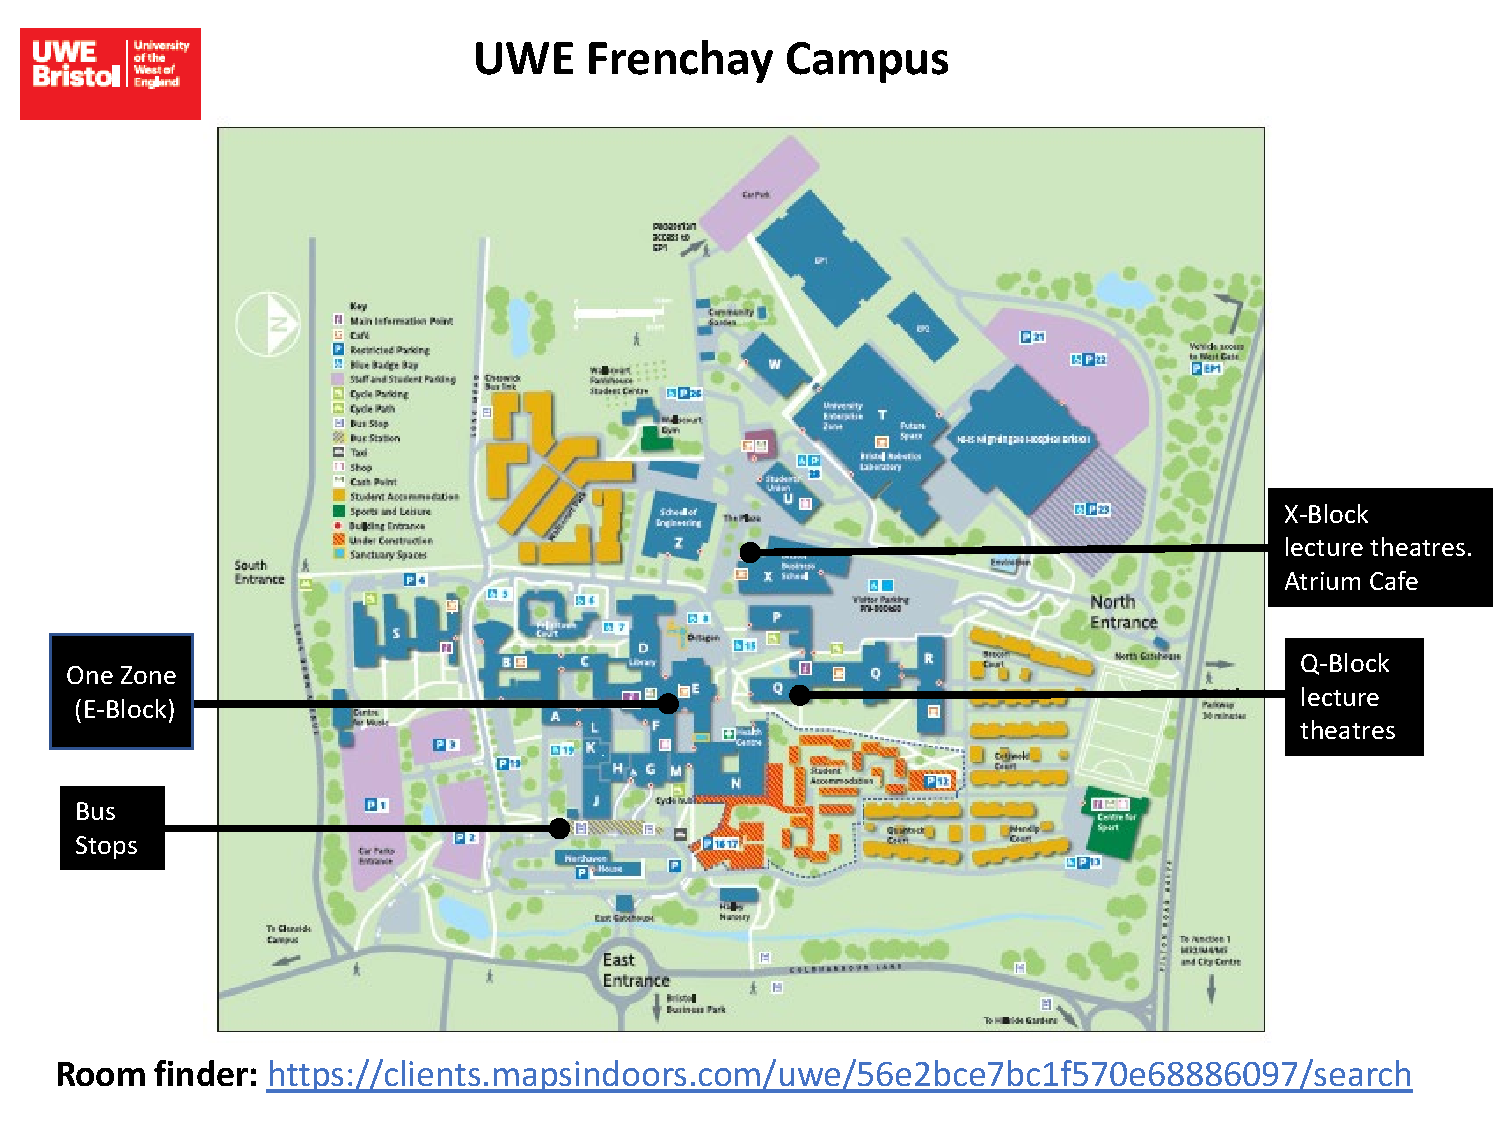
\includepdf[pages={-},fitpaper,rotateoversize]{Frenchay-Campus-Map.pdf}

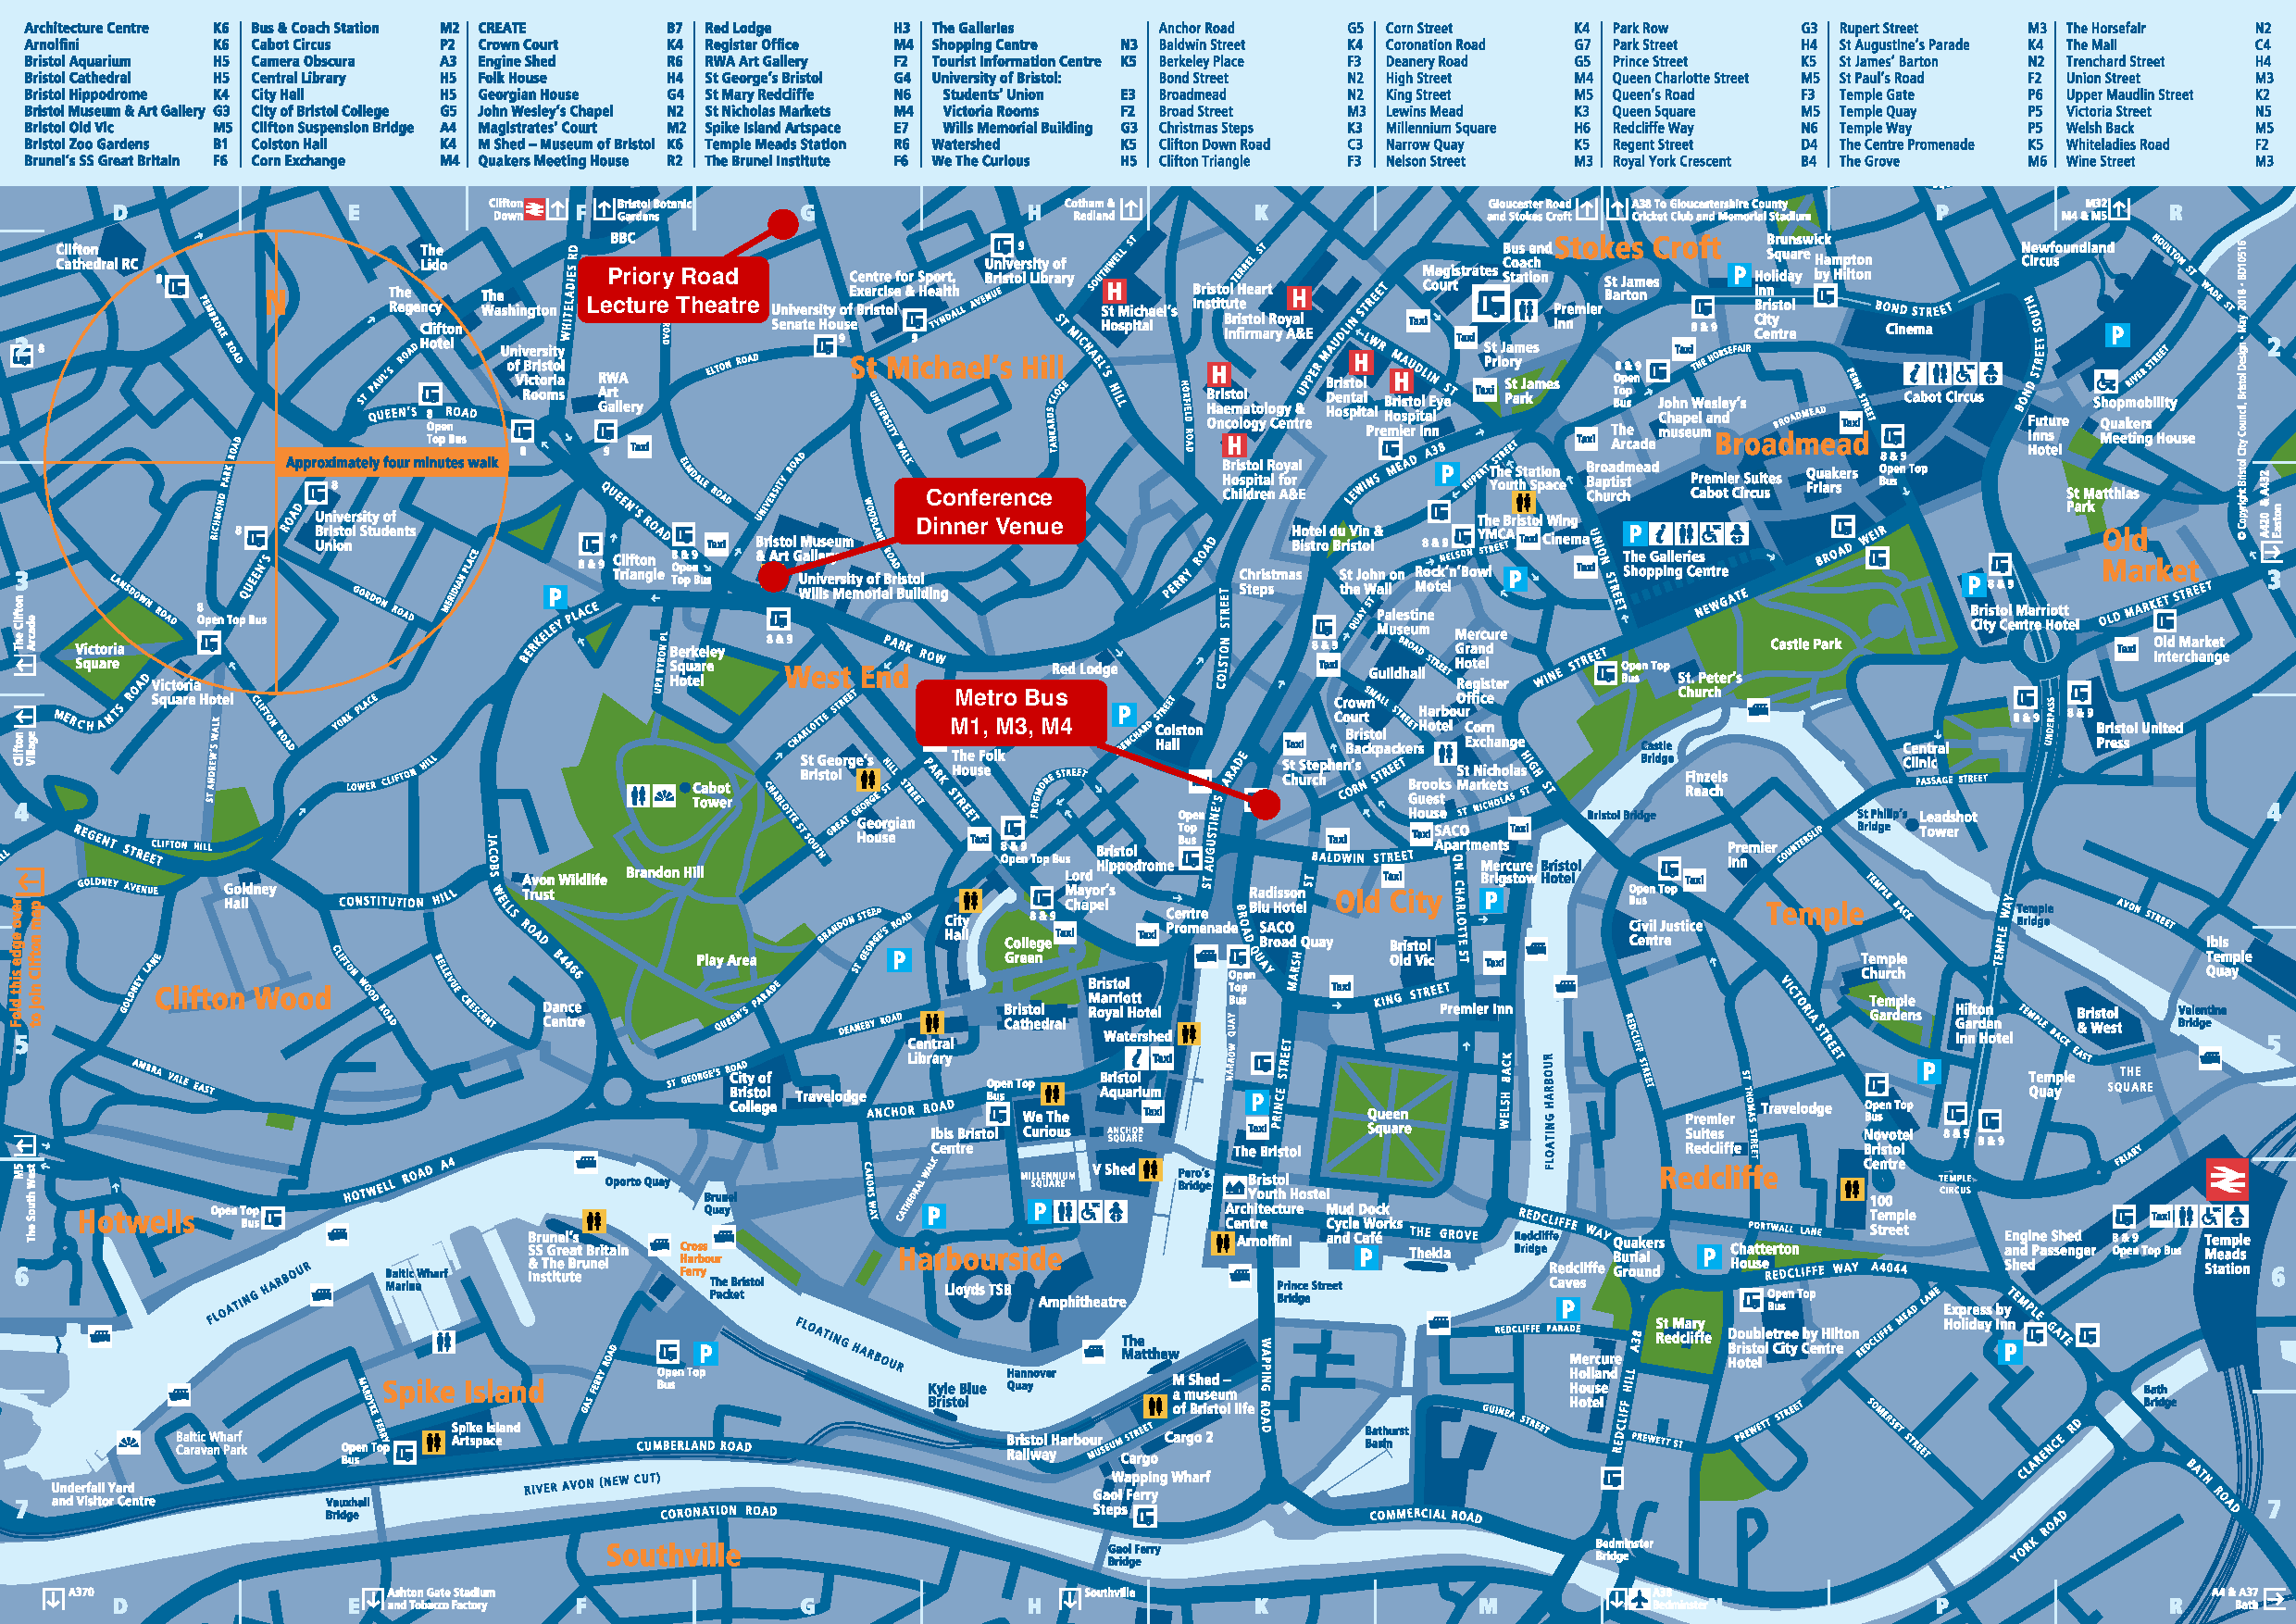
\includepdf[pages={-},fitpaper,rotateoversize]{Bristol-Map.pdf}

\end{document}
